\documentclass{jfp1}

\bibliographystyle{jfp}
% \citestyle{acmauthoryear}

\usepackage{bookmark}
\usepackage{booktabs}
\usepackage{subcaption}
\usepackage[utf8]{inputenc}
\usepackage[T1]{fontenc}
\usepackage{xspace}
\usepackage{fancyhdr}

% Haskell code snippets and useful shortcuts
\usepackage{minted}
\setminted[haskell]{escapeinside=@@}
\setminted[text]{escapeinside=@@}
\newcommand{\hs}{\mintinline{haskell}}
\newcommand{\cmd}[1]{\textsf{\color[rgb]{0,0,0.5} #1}}
\newcommand{\teq}{\smaller $\sim$}
\newcommand{\ghci}{$\lambda$>}
\newcommand{\defeq}{\stackrel{\text{def}}{=}}
\newcommand{\std}[1]{{\color[rgb]{0,0.3,0} #1}}
\newcommand{\blk}[1]{{\color[rgb]{0,0,0} #1}}
\newcommand{\blu}[1]{{\color[rgb]{0,0,0.5} #1}}
\newcommand{\gap}{$\;\;$}
\newcommand{\etal}{\emph{et~al.}}

% \renewcommand{\MintedPygmentize}{path-to-pygmentize}% Questions and tasks
\newcommand{\q}[2]{\textbf{\color{blue} Question (#1):} #2}
\newcommand{\todo}[2]{[\textbf{\color{red} #1:} #2]}

% Abbreviations for build systems
\newcommand{\Bazel}{\textsc{Bazel}\xspace}
\newcommand{\Buck}{\textsc{Buck}\xspace}
\newcommand{\Calc}{\textsc{Calc}\xspace}
\newcommand{\Cloud}{\textsc{Cloud}\xspace}
\newcommand{\CloudBuild}{\textsc{CloudBuild}\xspace}
\newcommand{\Dune}{\textsc{Dune}\xspace}
\newcommand{\Excel}{\textsc{Excel}\xspace}
\newcommand{\Fabricate}{\textsc{Fabricate}\xspace}
\newcommand{\Incremental}{\textsc{Incremental}\xspace}
\newcommand{\Make}{\textsc{Make}\xspace}
\newcommand{\Ninja}{\textsc{Ninja}\xspace}
\newcommand{\Nix}{\textsc{Nix}\xspace}
\newcommand{\Pluto}{\textsc{Pluto}\xspace}
\newcommand{\Redo}{\textsc{Redo}\xspace}
\newcommand{\Reflow}{\textsc{Reflow}\xspace}
\newcommand{\Shake}{\textsc{Shake}\xspace}
\newcommand{\Hadrian}{\textsc{Hadrian}\xspace}
\newcommand{\Tup}{\textsc{Tup}\xspace}
\newcommand{\store}{\hs{k}~\hs{->}~\hs{v}\xspace}
\newcommand{\storef}{\hs{k}~\hs{->}~\hs{f}~\hs{v}\xspace}

% \newcommand{\simon}[1]{}
% \newcommand{\simon}[1]{SLPJ: {\color{red} \em #1} End SLPJ}

\begin{document}
\title[Build Systems \`a la Carte: Theory and Practice]
{Build Systems \`a la Carte: Theory and Practice}

\author[Andrey Mokhov, Neil Mitchell and Simon Peyton Jones]
{ANDREY MOKHOV\\
School of Engineering, Newcastle University, United Kingdom}
\email{andrey.mokhov@ncl.ac.uk}

\author[Andrey Mokhov, Neil Mitchell and Simon Peyton Jones]
{NEIL MITCHELL\\
Digital Asset, United Kingdom}
\email{ndmitchell@gmail.com}

\author[Andrey Mokhov, Neil Mitchell and Simon Peyton Jones]
{SIMON PEYTON JONES\\
Microsoft Research, Cambridge, United Kingdom}
\email{simonpj@microsoft.com}

% \keywords{build systems, functional programming, algorithms}

\maketitle

\begin{abstract}
Build systems are awesome, terrifying -- and unloved. They are used by every
developer around the world, but are rarely the object of study. In this paper we
offer a systematic, and executable, framework for developing and comparing build
systems, viewing them as related points in a landscape rather than as isolated
phenomena. By teasing apart existing build systems, we can recombine their
components, allowing us to prototype new build systems with desired properties.
\end{abstract}

\section{Introduction}\label{sec-intro}

Build systems (such as \Make) are big, complicated, and used by every
software developer on the planet.  But they are a sadly unloved part
of the software ecosystem, very much a means to an end, and seldom the
focus of attention.
% Rarely do people ask questions like ``What does it mean for my build
% system to be correct?'' or ``What are the trade-offs between different
% approaches?''.
For years \Make dominated, but more recently the challenges of scale have driven
large software firms like Microsoft, Facebook and Google to develop their own
build systems, exploring new points in the design space. These complex build
systems use subtle algorithms, but they are often hidden away, and not the
object of study.

In this paper we give a general framework in which to understand and compare
build systems, in a way that is both abstract (omitting incidental detail) and
yet precise (implemented as Haskell code). Specifically we make these
contributions:

\begin{itemize}
\item Build systems vary on many axes, including: static vs dynamic
  dependencies; local vs cloud; deterministic vs non-deterministic build tasks;
  early cutoff; self-tracking build systems; and the type of persistently stored
  build information. In~\S\ref{sec-background} we identify some of these key
  properties, illustrated by four carefully-chosen build systems.

\item We describe some simple but novel abstractions that
  crisply encapsulate what a build system is (\S\ref{sec-abstractions}),
  allowing us, for example, to speak about what it means for a build system to
  be correct.

\item We identify two key design choices that are typically deeply wired into
  any build system: \emph{the order in which tasks are
  built}~(\S\ref{sec-scheduler}) and \emph{whether or not a
  task is rebuilt}~(\S\ref{sec-rebuilder}). These choices turn out to
  be orthogonal, which leads us to a new classification of the design
  space~(\S\ref{sec-design-space}).

\item We show that we can instantiate our abstractions to describe the essence
of a variety of different real-life build systems, including \Make, \Shake,
\Bazel, \Buck, \Nix, and \Excel\footnote{\Excel appears very different to the
others but, seen through the lens of this paper, it is very close.}, each by the
composition of the two design choices~(\S\ref{sec-implementations}). Doing this
modelling in a single setting allows the differences and similarities between
these huge systems to be brought out clearly\footnote{All our models are
executable and are available on Hackage as \cmd{build-1.0}.}.

\item Moreover, we can readily remix the ingredients to design new build systems
with desired properties, for example, to combine the advantages of \Shake and
\Bazel. Writing this paper gave us the insights to combine dynamic dependencies
and cloud build systems in a principled way; we evaluate the result
in~\S\ref{sec-experience}.

\item We can use the presented abstractions to more clearly explain details from
the original \Shake paper~(\S\ref{sec-step-traces}, \S\ref{sec-experience-shake})
and develop new cloud build features, which are already in use in industry and in
the GHC build system~(\S\S\ref{sec-using-cloud-shake}-\ref{sec-hadrian}).

\end{itemize}

In short, instead of seeing build systems as unrelated points in space, we now
see them as locations in a connected landscape, leading to a better
understanding of what they do and how they compare, and making it easier to
explore other points in the landscape. While we steer clear of many engineering
aspects of real build systems, in~\S\ref{sec-engineering} we discuss these
aspects in the context of the presented abstractions. The related work is covered
in~\S\ref{sec-related}.

This paper is an extended version of an earlier conference
paper~\cite{mokhov2018buildsystems}. The key changes compared to the earlier
version are: (i) we added further clarifications and examples
to~\S\ref{sec-abstractions}, in particular,~\S\ref{sec-task-examples} is
entirely new; (ii)~\S\ref{sec-scheduler} and~\S\ref{sec-rebuilder} are based on
the material from the conference paper but have been substantially expanded to
include further details and examples, as well as completely new material such
as~\S\ref{sec-step-traces}; (iii)~\S\ref{sec-experience} is completely new; (iv)
\S\ref{sec-failures} and \S\S\ref{sec-polymorphism}-\ref{sec-file-watching}
are almost entirely new, and \S\ref{sec-non-determinism} has been revised.
The new material focuses on our experience and various important practical
considerations, hence justifying the ``and Practice'' part of the paper title.

\section{Background}\label{sec-background}

Build systems automate the execution of repeatable tasks for individual users
and large organisations. In this section we explore the design space of build
systems, using four concrete examples: \Make~\cite{feldman1979make},
\Shake~\cite{mitchell2012shake}, \Bazel~\cite{bazel}, and
\Excel~\cite{advanced_excel}.
We have carefully chosen these four to illustrate the various axes on which
build systems differ; we discuss many other notable examples of build systems,
and their relationships, in~\S\ref{sec-implementations} and~\S\ref{sec-related}.

\subsection{The venerable \Make: static dependencies and file modification times}
\label{sec-background-make}

\Make\footnote{There are numerous implementations of \Make and none comes with a
formal specification. In this paper we therefore use a simple and sensible
approximation to a real \Make that you might find on your machine.} was developed
more than 40 years ago to automatically build software libraries and executable
programs from source code. It uses \emph{makefiles} to describe tasks (often
referred to as \emph{build rules}) and their dependencies in a simple textual form.
For example:

\vspace{1mm}
\begin{minted}[xleftmargin=10pt]{makefile}
util.o: util.h util.c
    gcc -c util.c
\end{minted}
\vspace{1mm}
\begin{minted}[xleftmargin=10pt]{makefile}
main.o: util.h main.c
    gcc -c main.c
\end{minted}
\vspace{1mm}
\begin{minted}[xleftmargin=10pt]{makefile}
main.exe: util.o main.o
    gcc util.o main.o -o main.exe
\end{minted}
\vspace{1mm}

\noindent
The above makefile lists three tasks: (i) compile a utility library comprising
files \cmd{util.h} and \cmd{util.c} into \cmd{util.o} by
executing\footnote{In this example we pretend \cmd{gcc} is a pure function for
the sake of simplicity. In reality, there are multiple versions of \cmd{gcc};
the actual binary used to compile and link files, and standard libraries
such that \cmd{stdio.h}, are often also listed as dependencies.} the command
\cmd{gcc -c util.c}, (ii) compile the main source file \cmd{main.c} into
\cmd{main.o}, and (iii) link object files \cmd{util.o} and \cmd{main.o} into the
executable \cmd{main.exe}. The makefile contains the complete information about
the \emph{task dependency graph}, which is shown in Fig.~\ref{fig-make}(a).

\begin{figure}[h]
\begin{subfigure}[b]{0.32\linewidth}
\centerline{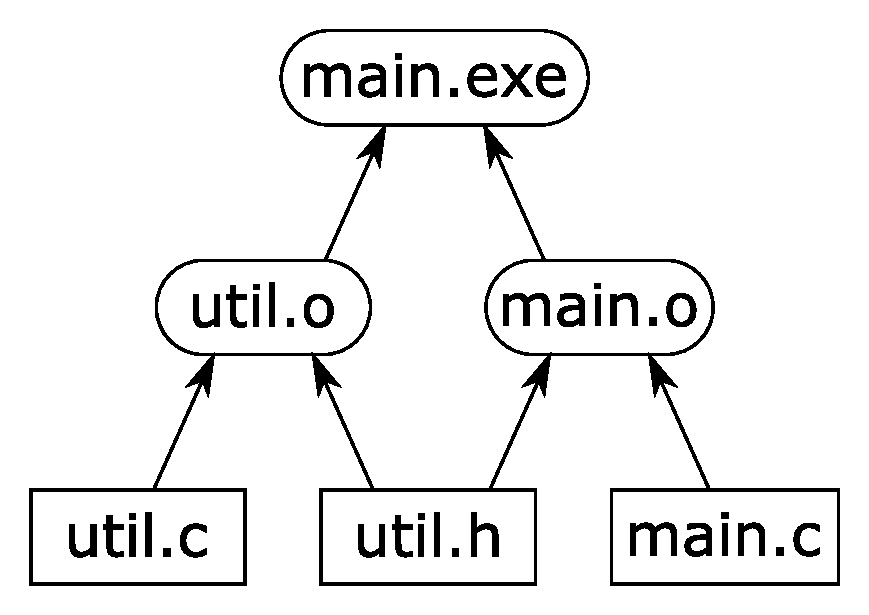
\includegraphics[scale=0.28]{fig/make-example.pdf}}
\caption{Task dependency graph}
\end{subfigure}
\begin{subfigure}[b]{0.32\linewidth}
\centerline{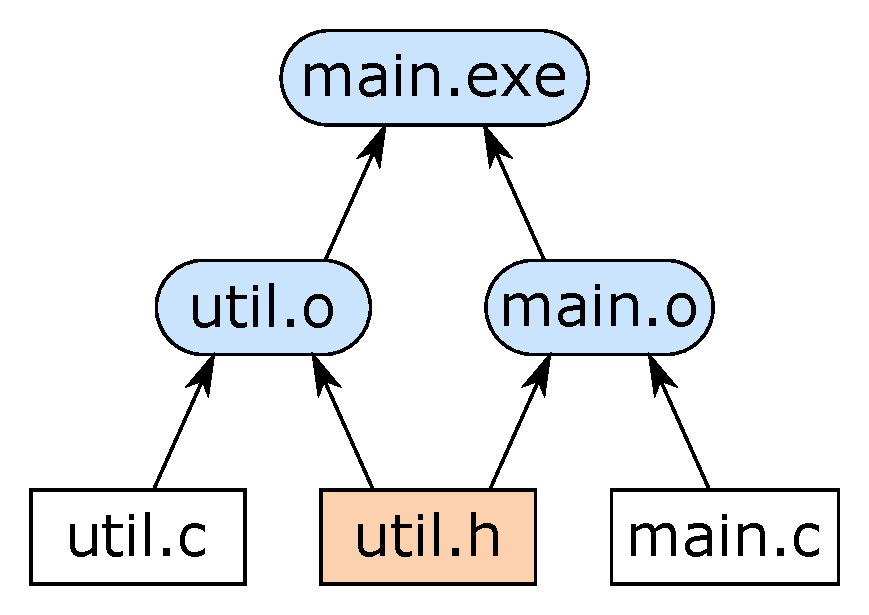
\includegraphics[scale=0.28]{fig/make-example-full.pdf}}
\caption{Full rebuild}
\end{subfigure}
\begin{subfigure}[b]{0.32\linewidth}
\centerline{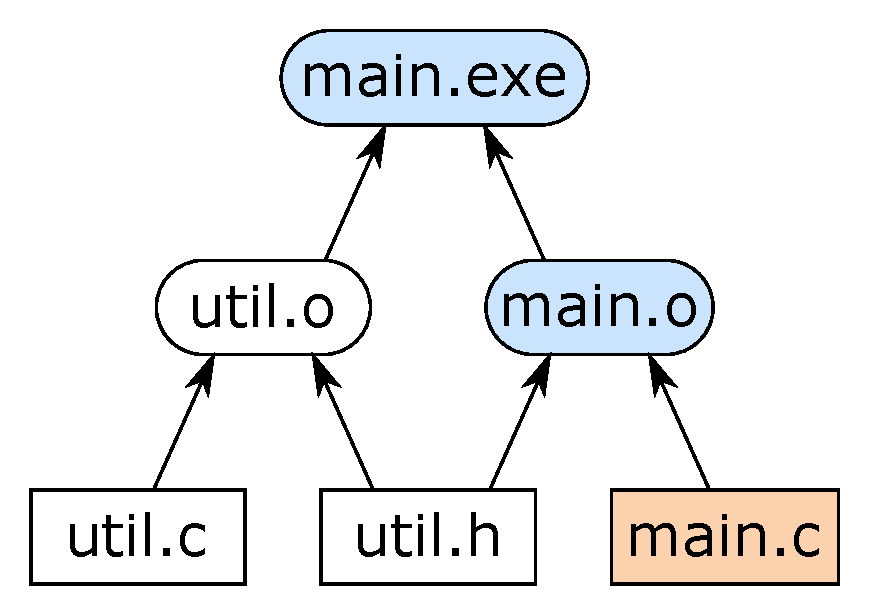
\includegraphics[scale=0.28]{fig/make-example-partial.pdf}}
\caption{Partial rebuild}
\end{subfigure}
\vspace{-2mm}
\caption{A task dependency graph and two build scenarios. Input files are shown
in rectangles, intermediate and output files are shown in rounded rectangles.
Modified inputs and files that are rebuilt are highlighted.
\label{fig-make}}
\vspace{-2mm}
\end{figure}

If the user runs \Make specifying \cmd{main.exe} as the desired output, \Make
will build~\cmd{util.o}~and~\cmd{main.o}, in any order since these tasks are
independent, and then \cmd{main.exe}. If the user modifies \cmd{util.h} and runs
\Make again, it will perform a \emph{full rebuild}, because all three tasks
transitively depend on \cmd{util.h}, as illustrated in Fig.~\ref{fig-make}(b).
On the other hand, if the user modifies \cmd{main.c} then a \emph{partial
rebuild} is sufficient: \cmd{util.o} does not need to be rebuilt, since its
inputs have not changed, see Fig.~\ref{fig-make}(c). Note that if the dependency
graph is \emph{acyclic} then each task needs to be executed at most once. Cyclic
task dependencies are typically not allowed in build systems but there are rare
exceptions, see~\S\ref{sec-iterative-compute}.

\noindent
The following property is essential for build systems; indeed, it is their
raison d'\^etre:

\definition[Minimality]{A build system is \emph{minimal} if it executes tasks at
most once per build and only if they transitively depend on inputs that changed
since the previous build.}\label{def-minimal}
\vspace{2mm}

To achieve minimality \Make relies on two main ideas: (i) it uses \emph{file
modification times} to detect which files changed\footnote{Technically, you
can fool \Make by altering the modification time of a file without changing its
content, e.g. by using the command \cmd{touch}. \Make is therefore minimal only
under the assumption that you do not do that.}, and (ii) it constructs a task
dependency graph from the information contained in the makefile and executes
tasks in a \emph{topological order}. For a more concrete description
see~\S\ref{sec-implementation-make}.

\subsection{\Excel: dynamic dependencies at the cost of minimality}
\label{sec-background-excel}

\Excel is a build system in disguise. Consider the following simple spreadsheet.

\vspace{1mm}
\begin{minted}[xleftmargin=10pt]{text}
A1: 10      B1: A1 + A2
A2: 20
\end{minted}
\vspace{1mm}

\noindent
There are two input cells \cmd{A1} and \cmd{A2}, and a single task that computes
the sum of their values, producing the result in cell \cmd{B1}. If either of
the inputs change, \Excel will recompute the result.

Unlike \Make, \Excel does not need to know all task dependencies upfront. Indeed, some
dependencies may change \emph{dynamically} according to computation results. For
example:

\vspace{1mm}
\begin{minted}[xleftmargin=10pt]{text}
A1: 10      B1: INDIRECT("A" & C1)      C1: 1
A2: 20
\end{minted}
\vspace{1mm}

\noindent
The formula in \cmd{B1} uses the \cmd{INDIRECT} function, which takes a string
and returns the value of the cell with that name.  The string evaluates to
\cmd{"A1"}, so \cmd{B1} evaluates to \cmd{10}. However, the dependencies of the
formula in \cmd{B1} are determined by the value of \cmd{C1}, so it is impossible
to compute the dependency graph before the build starts\footnote{In
this particular example one might say that the value of
\cmd{C1} is statically known, but imagine that it is the result of a long
computation chain -- its value will only become available during the build.}.

To support dynamic dependencies, \Excel's calc engine~\cite{excel_recalc} is
significantly different from \Make. \Excel arranges the cells into a linear
sequence, called the \emph{calc chain}.  During the build, \Excel processes
cells in the calc-chain sequence, but if computing a cell \cmd{C} requires the
value of a cell \cmd{D} that has not yet been computed, \Excel \emph{aborts}
computation of \cmd{C}, moves \cmd{D} before \cmd{C} in the calc chain, and
resumes the build starting with \cmd{D}. When a build is complete, the resulting
calc chain respects all the dynamic dependencies of the spreadsheet. When an
input value (or formula) is changed, \Excel uses the final calc chain from the
\emph{previous} build as its starting point so that, in the common case where
changing an input value does not change dependencies, there are no aborts.
Notice that build always succeeds regardless of the initial calc chain (barring
truly circular dependencies); the calc chain is just an optimisation.
We refer to this algorithm as \emph{restarting}, and discuss it
in more detail in~\S\ref{sec-implementation-excel}.

Dynamic dependencies complicate minimality.  In the above example, \cmd{B1}
should only be recomputed if \cmd{A1} or \cmd{C1} change, but not if (say)
\cmd{A2} changes; but these facts are not statically apparent. In practice
\Excel implements a conservative approximation to minimality: it recomputes a
formula if~(i)~the formula statically mentions a changed cell, or~(ii)~the formula uses a
function like \cmd{INDIRECT} whose dependencies are not statically visible,
or~(iii)~the formula itself has changed.

Item (iii) in the above list highlights another distinguishing feature of \Excel: it
is \emph{self-tracking}. Most build systems only track changes of inputs and
intermediate results, but \Excel also tracks changes in the tasks themselves: if
a formula is modified, \Excel will recompute it and propagate the changes.
Self-tracking is uncommon in software build systems, where one often needs to
manually initiate a full rebuild even if just a single task has changed.
We discuss self-tracking further in~\S\ref{sec-tracking-aspects}.

\begin{figure}
\begin{subfigure}[b]{0.90\linewidth}
\centerline{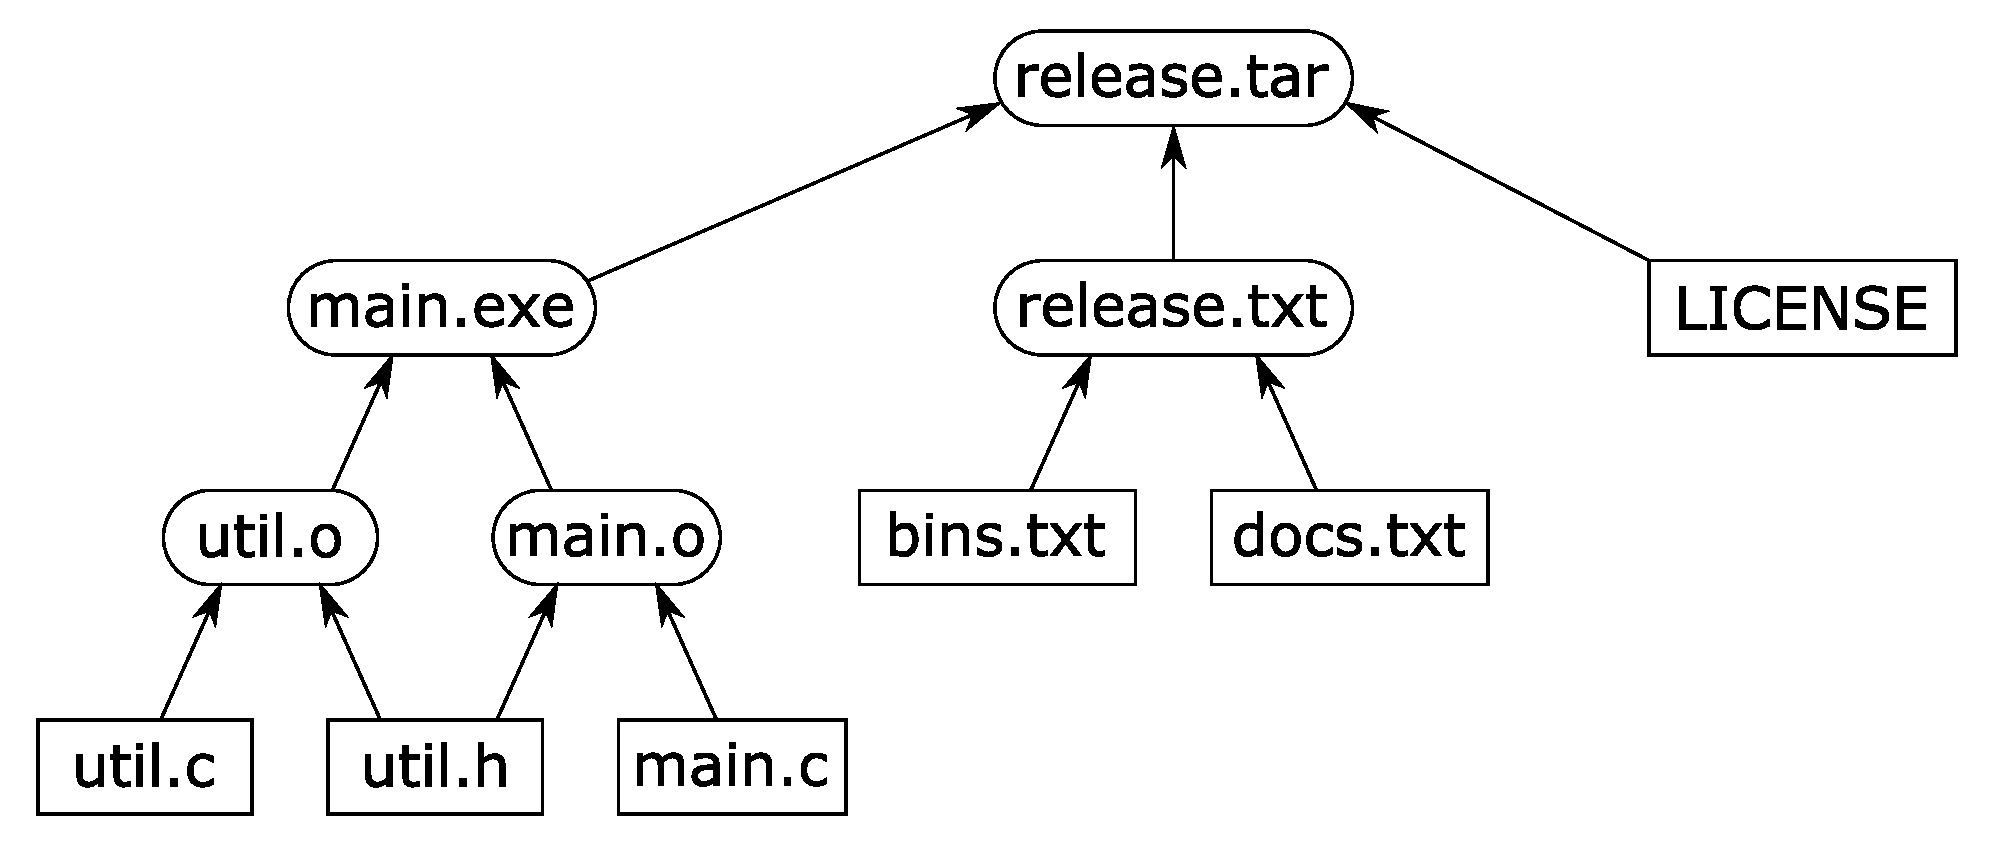
\includegraphics[scale=0.28]{fig/shake-example.pdf}}
\caption{Dependency graph produced after the previous build.}
\end{subfigure}
\begin{subfigure}[b]{0.90\linewidth}
\centerline{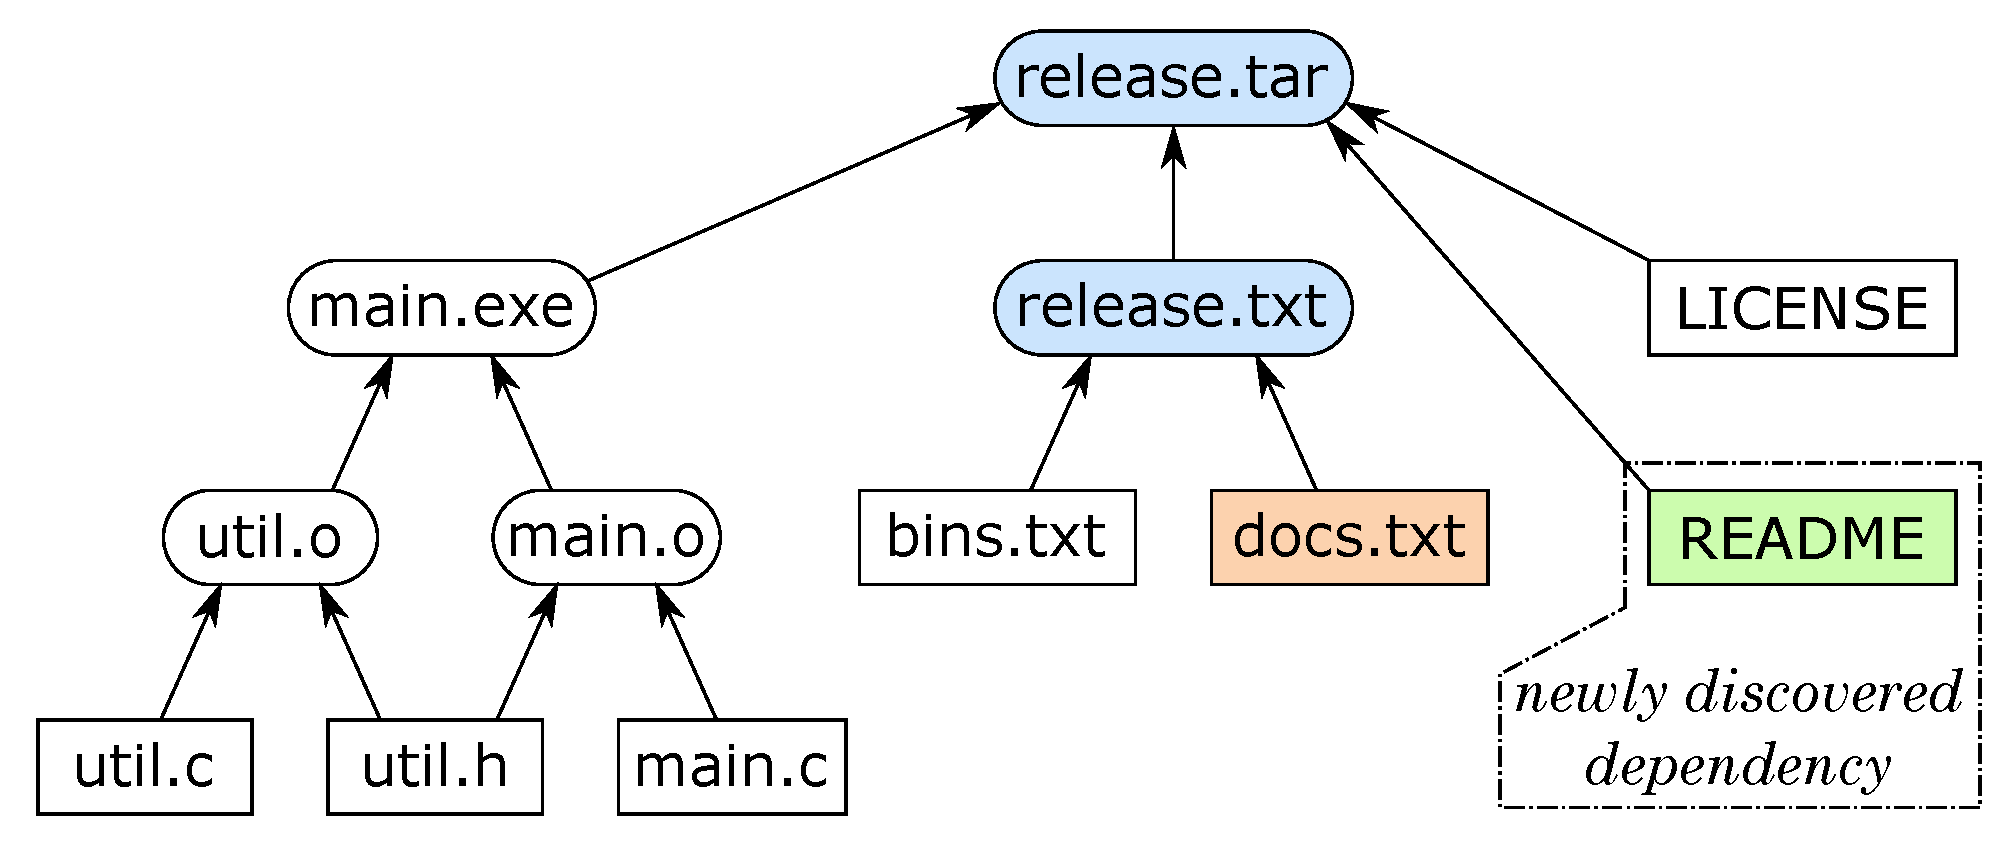
\includegraphics[scale=0.28]{fig/shake-example-rebuild.pdf}}
\caption{Since \cmd{docs.txt} was modified, we rebuild \cmd{release.txt} and
\cmd{release.tar}, discovering a new dependency.}
\end{subfigure}
\vspace{-2mm}
\caption{Dynamic dependencies example: create \cmd{README} and add it to the
list of release documents \cmd{docs.txt}.\label{fig-shake}}
\vspace{-4mm}
\end{figure}

\subsection{\Shake: dynamic dependencies with no remorse}
\label{sec-background-shake}

\Shake was developed to solve the issue of dynamic
dependencies~\cite{mitchell2012shake} without sacrificing
the minimality requirement. Building on the \Make example
from~\S\ref{sec-background-make}, we add the following files whose
dependencies are shown in Fig.~\ref{fig-shake}(a):

\begin{itemize}
    \item \cmd{LICENSE} is an input text file containing the project license.
    \item \cmd{release.txt} is a text file listing all files that should be in the release. This file
    is produced by concatenating input files \cmd{bins.txt} and \cmd{docs.txt},
    which list all binary and documentation files of the project.
    \item \cmd{release.tar} is the release archive built by executing the
    command \cmd{tar} on the release files.
\end{itemize}

The dependencies of \cmd{release.tar} are not known statically: they are
determined by the content of \cmd{release.txt}, which might not even exist
before the build. Makefiles cannot express such dependencies, requiring problematic
workarounds such as \emph{build phases} \cite{hadrian}.
In \Shake we can express the rule for \cmd{release.tar} as:

\begin{minted}[xleftmargin=10pt]{haskell}
"release.tar" %> \_ -> do
    need ["release.txt"]
    files <- lines <$> readFile "release.txt"
    need files
    system "tar" $ ["-cf", "release.tar"] ++ files
\end{minted}

\noindent
We first declare the static dependency on \cmd{release.txt}, then read its
content (a list of files) and depend on each listed file, dynamically. Finally, we specify the
command to produce the resulting archive. Crucially, the archive will only be
rebuilt if one of the dependencies (static or dynamic) has changed. For example,
if we create another documentation file \cmd{README} and add it to
\cmd{docs.txt}, \Shake will appropriately rebuild \cmd{release.txt} and
\cmd{release.tar}, discovering the new dependency, see Fig.~\ref{fig-shake}(b).

\Shake's implementation is different from both \Make and \Excel in two aspects.
First, it uses the dependency graph from the previous build to decide which
files need to be rebuilt. This idea has a long history, going back to
\emph{incremental}~\cite{demers1981incremental},
\emph{adaptive}~\cite{acar2002adaptive}, and
\emph{self-adjusting computations} (see \cite{acar2007selfadjusting} and
\S\ref{sec-related}). Second, instead of aborting and deferring the execution of
tasks whose newly discovered dependencies have not yet been built (as \Excel
does), \Shake \emph{suspends} their execution until the dependencies are brought
up to date. We refer to this task scheduling algorithm as \emph{suspending},
see a concrete implementation in~\S\ref{sec-implementation-shake}.

\begin{figure}
\vspace{-3mm}
\centerline{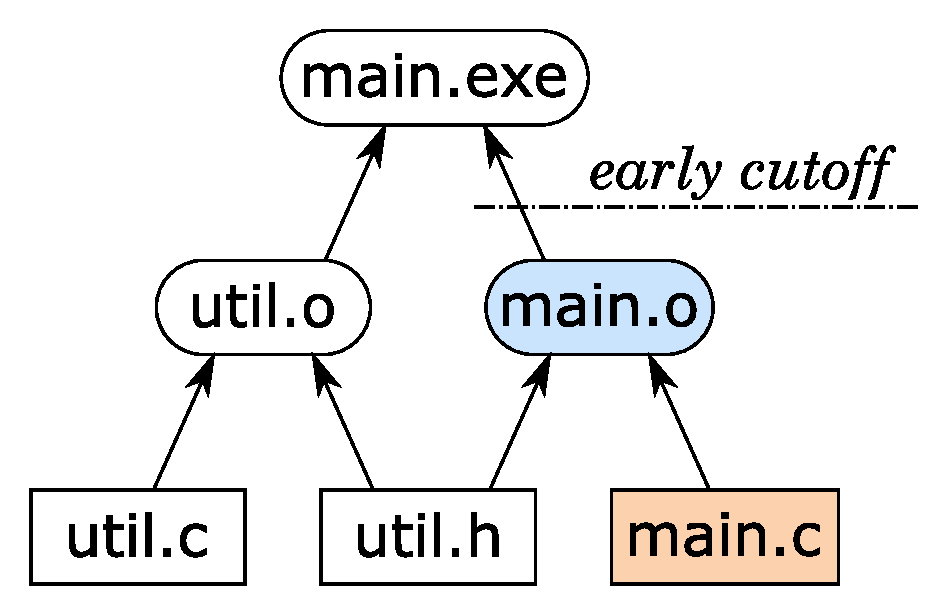
\includegraphics[scale=0.28]{fig/shake-example-cutoff.pdf}}
\vspace{-4mm}
\caption{An early cutoff example: if a comment is added to \cmd{main.c}, the
rebuild is stopped after detecting that \cmd{main.o} is unchanged, since this
indicates that \cmd{main.exe} and its dependents do not need to be
rebuilt.\label{fig-cutoff}}
\vspace{-4mm}
\end{figure}

\Shake also supports the \emph{early cutoff optimisation}. When it
executes a task and the result is unchanged from the previous build, it is
unnecessary to execute the dependent tasks, and hence \Shake can stop a build
earlier, as illustrated in Fig.~\ref{fig-cutoff}. Not all build systems support
early cutoff: \Make and \Excel do not, whereas \Shake and \Bazel (introduced
below) do.

\vspace{-0.5mm}
\subsection{\Bazel: a cloud build system}\label{sec-background-bazel}
\vspace{-0.5mm}

When build systems are used by large teams, different team members often end up
executing exactly the same tasks on their local machines. A \emph{cloud build
system} can speed up builds dramatically by sharing build results
among team members. Furthermore, cloud build systems can support \emph{shallow
builds} that materialise only end build products locally, leaving all
intermediates in the cloud.

Consider an example in Fig.~\ref{fig-bazel}. The user starts by downloading the
sources, whose content hashes are (for simplicity)~1,~2 and~3, and requests to
build \cmd{main.exe}, see Fig.~\ref{fig-bazel}(a,b). By looking up the global
history of all previous builds\footnote{In practice, old entries are regularly
evicted from the cloud storage, as further discussed
in~\S\ref{sec-cloud-aspects}.}, the build system finds that someone has already
compiled these exact sources before and the resulting files \cmd{util.o} and
\cmd{main.o} had hashes 4~and~5, respectively. Similarly, the build system finds
that the hash of the resulting \cmd{main.exe} was 6 and downloads the actual
binary from the cloud storage -- it must be materialised, because it is the end
build product.

In Fig.~\ref{fig-bazel}(c), the user modifies the source file \cmd{util.c},
thereby changing its hash from~1~to~7. The cloud lookup of the new combination
$\{\cmd{util.c}, \cmd{util.h}\}$ fails, which means that nobody has ever
compiled it. The build system must therefore build \cmd{util.o}, materialising
it with the new hash~8. The combination of hashes of \cmd{util.o} and
\cmd{main.o} has not been encountered before either, thus the build system first
downloads \cmd{main.o} from the cloud and then builds \cmd{main.exe} by linking
the two object files. When the build is complete, the results can be uploaded to
the cloud for future reuse by other team members.

\Bazel is one of the first openly-available cloud build systems.
As of writing, it is not possible to express dynamic dependencies in
user-defined build rules; however some of the pre-defined build rules require
dynamic dependencies and the internal build engine can cope with them by using
a \emph{restarting} task scheduler, which is similar to that of \Excel but does
not use the calc chain. \Bazel is not minimal in the sense that it may restart a
task multiple times as new dependencies are discovered and rebuilt, but it
supports the early cutoff optimisation.

To support cloud builds, \Bazel maintains (i) a \emph{content-addressable cache}
that can be used to download a previously built file given the hash of its
content, and (ii) the history of all executed build commands annotated with
observed file hashes. The latter allows the build engine to bypass the execution
of a task, by predicting the hash of the result from the hashes of its
dependencies, and subsequently download the result from the cache. A concrete
implementation is provided in~\S\ref{sec-implementation-cloud}.

\begin{figure}
\vspace{-2mm}
\begin{subfigure}[b]{0.25\linewidth}
\centerline{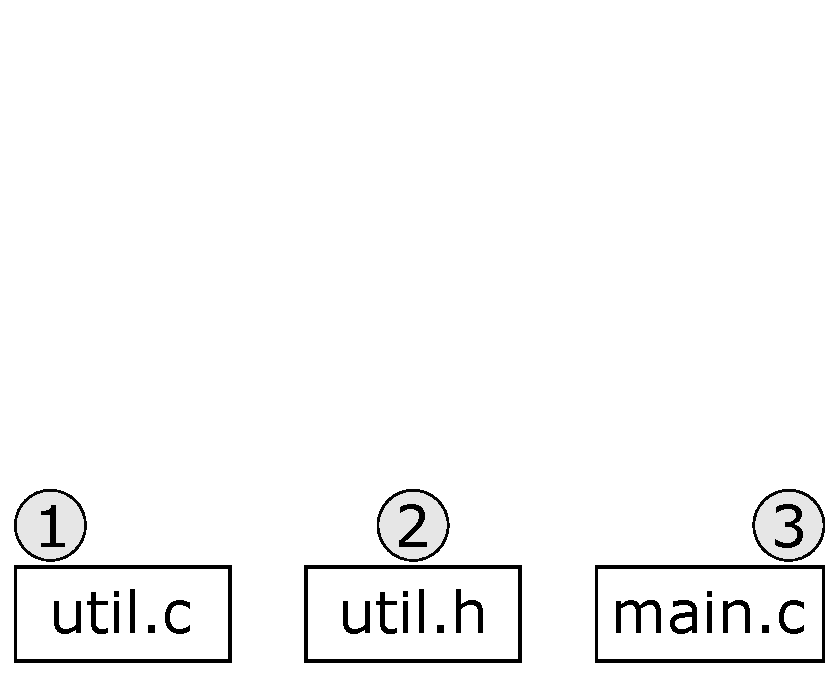
\includegraphics[scale=0.28]{fig/bazel-example-checkout.pdf}}
\vspace{-1mm}
\caption{Download source files}
\end{subfigure}
\begin{subfigure}[b]{0.40\linewidth}
\centerline{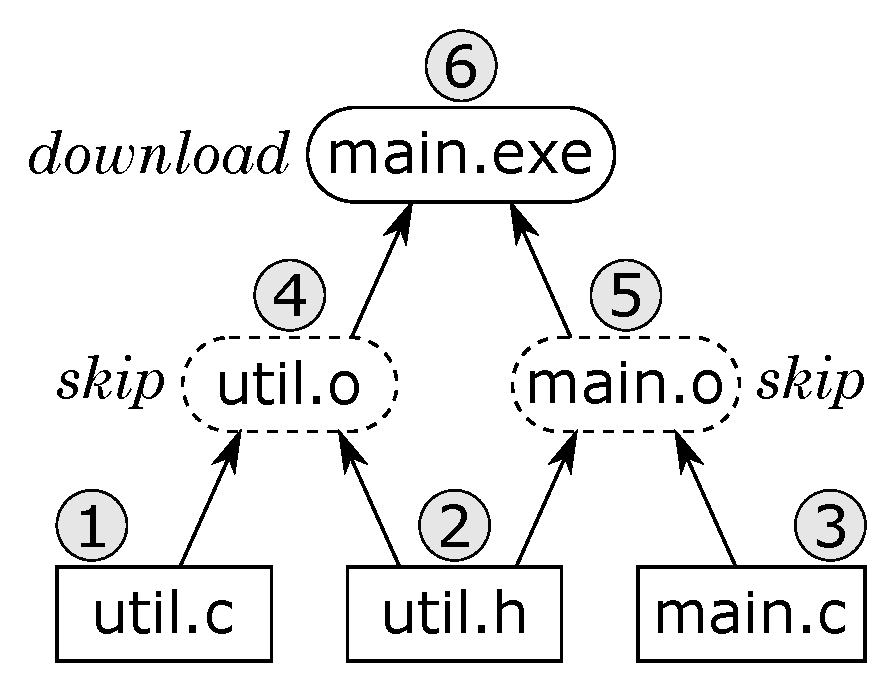
\includegraphics[scale=0.28]{fig/bazel-example-build.pdf}}
\vspace{-1mm}
\caption{Build \cmd{main.exe}}
\end{subfigure}
\begin{subfigure}[b]{0.31\linewidth}
\centerline{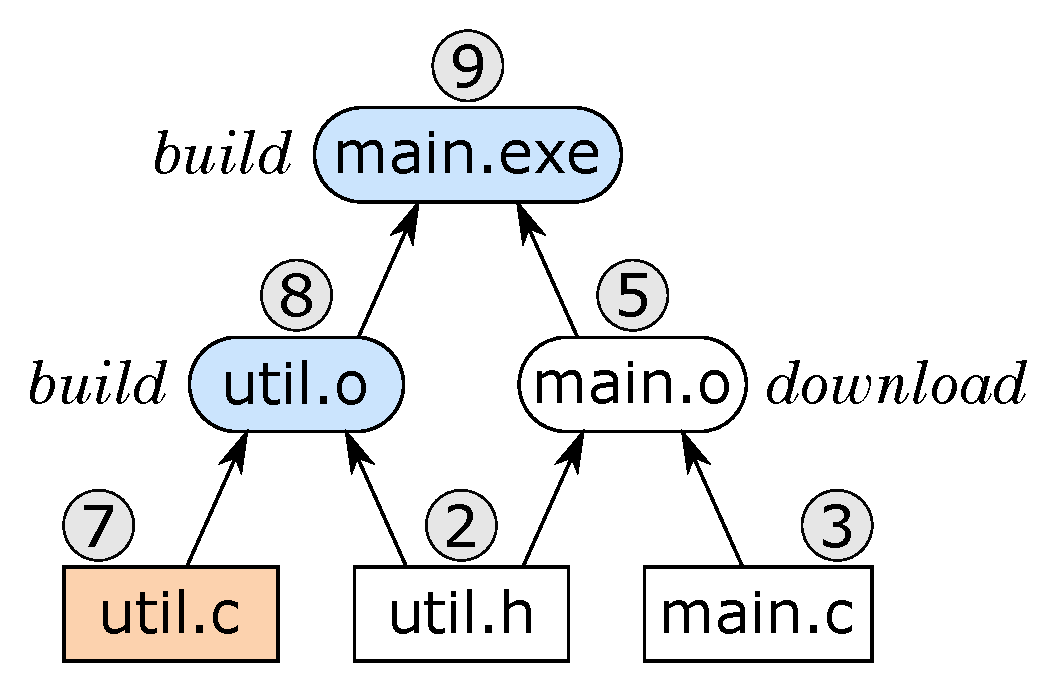
\includegraphics[scale=0.28]{fig/bazel-example-rebuild.pdf}}
\vspace{-1mm}
\caption{Modify \cmd{util.c} and rebuild}
\end{subfigure}
\vspace{-2.5mm}
\caption{A cloud build example: (a)~download sources, (b)~build \cmd{main.exe}
by downloading it from the cloud and skipping intermediate files (only their
hashes are needed), (c)~modify \cmd{util.c} and rebuild \cmd{main.exe}, which
requires building \cmd{util.o} (nobody has compiled \cmd{util.c} before) and
downloading \cmd{main.o} (it is needed for linking \cmd{main.exe}). File hashes
are shown in circles, and non-materialised intermediates in dashed rounded
rectangles.\label{fig-bazel}}
\vspace{-3mm}
\end{figure}

\begin{table}[h]
\vspace{-1mm}
\smaller
\centering
\begin{tabular}{l||l|l||l|c|c|c}
\hline
$\!$Build system$\!$& Persistent build information & Scheduler   & Dependencies    & Minimal & Cutoff & Cloud$\!$\\\hline
$\!$\Make       $\!$& File modification times      & Topological & Static          & Yes     & No     & No   $\!$\\
$\!$\Excel      $\!$& Dirty cells, calc chain      & Restarting  & Dynamic         & No      & No     & No   $\!$\\
$\!$\Shake      $\!$& Previous dependency graph    & Suspending  & Dynamic         & Yes     & Yes    & No   $\!$\\
$\!$\Bazel      $\!$& Cloud cache, command history & Restarting  & Dynamic$^{(*)}$ & No      & Yes    & Yes  $\!$\\\hline
\hline
\end{tabular}
\caption{Build system differences; $^{(*)}$at present, user-defined build rules
cannot have dynamic dependencies.\label{tab-summary}}
\vspace{-8mm}
\end{table}

\vspace{-1.5mm}
\subsection{Summary}\label{sec-background-summary}
\vspace{-0.5mm}

We summarise differences between four discussed build systems in
Table~\ref{tab-summary}. The column \emph{`persistent build information'} refers
to the information that build systems persistently store between builds:
\begin{itemize}
    \item \Make stores file modification times, or rather, it relies on the file
    system to do that.
    \item \Excel stores one dirty bit per cell and the calc chain from the
    previous build.
    \item \Shake stores the dependency graph discovered in the previous build,
    annotated with file content hashes for efficient checking of file changes.
    \item \Bazel stores the content-addressable cache and the history of all
    previous build commands annotated with file hashes. This information is
    shared among all users of the build system.
\end{itemize}

In this paper we elucidate which build system properties are consequences of
specific implementation choices (stored metadata and task scheduling algorithm),
and how one can obtain new build systems with desired properties by recombining
parts of existing implementations. As a compelling example,
in~\S\ref{sec-implementation-cloud} we demonstrate how to combine the advantages
of \Shake and \Bazel.

\section{Build systems, abstractly}\label{sec-abstractions}

This section presents purely functional abstractions that allow us to express
all the intricacies of build systems discussed in the previous
section~\S\ref{sec-background} and design complex build systems from simple
primitives. Specifically, we present the \emph{task} and \emph{build}
abstractions in~\S\ref{sec-task} and~\S\ref{sec-general-build}, respectively.
Sections~\S\ref{sec-build} and~\S\ref{sec-implementations} scrutinise the
abstractions further and provide concrete implementations for several build
systems.

\subsection{Common vocabulary for build systems}\label{sec-vocabulary}
\begin{figure}
\begin{minted}[fontsize=\small]{haskell}
-- An abstract store
data Store i k v
getInfo    :: Store i k v -> i
putInfo    :: Store i k v -> i -> Store i k v
getValue   :: Store i k v -> k -> v
putValue   :: Eq k => Store i k v -> k -> v -> Store i k v
getHash    :: Hashable v => Store i k v -> k -> Hash v
initialise :: i -> (k -> v) -> Store i k v
\end{minted}
\vspace{1mm}
\begin{minted}[fontsize=\small]{haskell}
-- Hashing
hash :: Hashable a => a -> Hash a
\end{minted}
\vspace{1mm}
\begin{minted}[fontsize=\small]{haskell}
-- Applicative functors
pure  :: Applicative f => a -> f a
(<$>) :: Applicative f =>   (a -> b) -> f a -> f b -- Left-associative
(<*>) :: Applicative f => f (a -> b) -> f a -> f b -- Left-associative
\end{minted}
\vspace{1mm}
\begin{minted}[fontsize=\small]{haskell}
-- Standard State monad from Control.Monad.State
data State s a
instance Applicative (State s)
instance Monad       (State s)
get       :: State s s
put       :: s -> State s ()
modify    :: (s -> s) -> State s ()
execState :: State s a -> s -> s
\end{minted}
\vspace{1mm}
\begin{minted}[fontsize=\small]{haskell}
-- Standard types from Data.Functor.Identity and Data.Functor.Const
newtype Identity a = Identity { runIdentity :: a }
newtype Const m a  = Const    { getConst    :: m }
\end{minted}
\vspace{0.5mm}
\begin{minted}[fontsize=\small]{haskell}
instance Functor (Const m) where
    fmap _ (Const m) = Const m
\end{minted}
\vspace{0.5mm}
\begin{minted}[fontsize=\small]{haskell}
instance Monoid m => Applicative (Const m) where
    pure _              = Const mempty
    Const x <*> Const y = Const (x <> y)
\end{minted}
\vspace{-3mm}
\caption{Signatures of main data types and library functions.}\label{fig-types}
\vspace{-4mm}
\end{figure}
We  begin by establishing a common vocabulary for build systems.

\vspace{-2mm}
\paragraph{Keys, values, and the store} The goal of any build system is to
bring up to date a \emph{store} that implements a mapping from \emph{keys} to
\emph{values}. In software build systems the store is the file system, the
keys are filenames, and the values are file contents. In \Excel, the store is
the worksheets, the keys are cell names (such as \cmd{A2}) and the values are
numbers, strings etc, displayed as the cell contents. Many systems use
\emph{hashes} of values as compact summaries with a fast equality check.

\vspace{-2mm}
\paragraph{Input, output, and intermediate values}
Some values must be provided by the user as \emph{input}. For example,
\cmd{main.c} can be edited by the user who relies on the build system to
compile it into \cmd{main.o} and subsequently \cmd{main.exe}. End build products,
such as \cmd{main.exe}, are \emph{output} values. All other values (in this case
\cmd{main.o}) are \emph{intermediate}; they are not interesting for the user
but are produced in the process of turning inputs into outputs.

\vspace{-2mm}
\paragraph{Persistent build information} As well as the key/value mapping, the store
also contains information maintained by the build system itself, which persists
from one invocation of the build system to the next -- its ``memory''.

\paragraph{Task description} Any build system requires the user to specify how to
compute the new value for one key, using the (up to date) values of its
dependencies. We call this specification the \emph{task description}.  For
example, in \Excel, the formulae of the spreadsheet constitute the task
description; in \Make the rules in the makefile are the task description.

\vspace{-2mm}
\paragraph{Build system} A \emph{build system} takes a task description, a target
key, and a store, and returns a new store in which the target key has an
up to date value.

\vspace{-2mm}
\paragraph{Modelling in Haskell} We will model all our build systems concretely,
as Haskell programs. To that end, Fig.~\ref{fig-types} gives the type
declarations and function signatures of the library functions. For example,
\hs{Store}~\hs{i}~\hs{k}~\hs{v} is the type of stores, with several associate
functions (\hs{getValue}, etc.). We use \hs{k} as a type
variable ranging over keys, \hs{v} for values, and \hs{i} for the persistent
build information.

\subsection{The Task abstraction}\label{sec-task}

Our first main abstraction is for \emph{task descriptions}:
\begin{minted}[xleftmargin=10pt]{haskell}
type Task c k v = @\std{forall}@ f. c f => (k -> f v) -> k -> Maybe (f v)
\end{minted}
This highly-abstracted type\footnote{Readers familiar with \emph{lenses} or
\emph{profunctor optics} might recognise a familiar pattern. We discuss this
in~\S\ref{sec-related-optics}.} is best introduced by an example.
Consider this \Excel spreadsheet:
\vspace{1mm}
\begin{minted}[xleftmargin=10pt]{text}
A1: 10     B1: A1 + A2
A2: 20     B2: B1 * 2
\end{minted}
\vspace{1mm}
Here cell \cmd{A1} contains the value \cmd{10}, the cell \cmd{B1} contains
the formula \cmd{A1+A2}, etc. We can represent the formulae of this spreadsheet
with the following task description:
\vspace{1mm}
\begin{minted}[xleftmargin=10pt]{haskell}
sprsh1 :: Task Applicative String Integer
sprsh1 fetch "B1" = Just ((+)   <$> fetch "A1" <*> fetch "A2")
sprsh1 fetch "B2" = Just ((* 2) <$> fetch "B1")
sprsh1 _     _    = Nothing
\end{minted}
\vspace{1mm}
Here we instantiate keys \hs{k} with \hs{String}, and values \hs{v} with \hs{Integer}.
(Real spreadsheet cells would contain a wider range of values, of course.)
The task description \hs{sprsh1} embodies all the \emph{formulae} of the spreadsheet,
but not the input values.  Like every \hs{Task}, \hs{sprsh1} is given a
\emph{callback} \hs{fetch} and a key. It pattern-matches on the key to see if it
has a task description (in the \Excel case, a formula) for it. If not, it returns
\hs{Nothing}, indicating the key is an input. If there is a formula in the cell,
it computes the value of the formula, using \hs{fetch} to find the value of any
keys on which it depends.

The code to ``compute the value of a formula'' in \hs{sprsh1} looks a bit mysterious
because it takes place in an \hs{Applicative} computation \cite{mcbride2008applicative}
-- the relevant type signatures are given in Fig.~\ref{fig-types}. We will
explain why in subsection~\S\ref{sec-general-build}.

For now, we content ourselves with observing that a task description,
of type \hs{Task}~\hs{c}~\hs{k}~\hs{v}, is completely isolated from the world of
compilers, calculation chains, file systems, caches, and all other
complexities of real build systems.  It just computes a single output, in
a side-effect-free way, using a callback (\hs{fetch}) to find the values
of its dependencies.

\subsection{The Build abstraction}\label{sec-general-build}

Next comes our second main abstraction -- a build system:
\vspace{1mm}
\begin{minted}[xleftmargin=10pt]{haskell}
type Build c i k v = Task c k v -> k -> Store i k v -> Store i k v
\end{minted}
\vspace{1mm}
The signature is very straightforward.  Given a task description, a target key,
and a store, the build system returns a new store in which the value of the
target key is up to date. What exactly does ``up to date'' mean?  We answer
that precisely in \S\ref{sec-build-correctness}.

\noindent
Here is a simple build system:
\vspace{1mm}
\begin{minted}[xleftmargin=10pt]{haskell}
busy :: Eq k => Build Monad () k v
busy task key store = execState (fetch key) store
  where
    fetch :: k -> State (Store i k v) v
    fetch k = case task fetch k of
        Nothing  -> do s <- get; return (getValue s k)
        Just act -> do v <- act; modify (\s -> putValue s k v); return v
\end{minted}
\vspace{1mm}

\noindent
The \hs{busy} build system defines the callback \hs{fetch} so that, when given a
key, it brings the key up to date in the store, and returns its value.
The function \hs{fetch} runs in the standard Haskell \hs{State} monad -- see
Fig.~\ref{fig-types} -- initialised with the incoming \hs{store} by \hs{execState}.
To bring a key up to date, \hs{fetch} asks the task description \hs{task} how
to compute \hs{k}. If \hs{task} returns \hs{Nothing} the key is an input, so
\hs{fetch} simply reads the result from the store. Otherwise \hs{fetch} runs
the action \hs{act} returned by the \hs{task} to produce a resulting
value~\hs{v}, records the new key/value mapping in the store, and returns \hs{v}.
Notice that \hs{fetch} passes itself to \hs{task} as an argument, so that the
latter can use \hs{fetch} to recursively find the values of \hs{k}'s dependencies.

Given an acyclic task description, the \hs{busy} build system terminates with a
correct result, but it is not a \emph{minimal} build system
(Definition~\ref{def-minimal}). Since \hs{busy} has no memory
(\hs{i}~\hs{=}~\hs{()}), it cannot keep track of keys it has already built, and
will therefore busily recompute the same keys again and again if they have
multiple dependents. We will develop much more efficient build systems
in~\S\ref{sec-implementations}.

Nevertheless, \hs{busy} can easily handle the example \hs{sprsh1}
from the previous subsection~\S\ref{sec-task}. In the GHCi session below we
initialise the store with \cmd{A1} set to 10 and all other cells set to 20.

\begin{minted}[xleftmargin=10pt]{haskell}
@\ghci@ store  = initialise () (\key -> if key == "A1" then 10 else 20)
@\ghci@ result = busy sprsh1 "B2" store
@\ghci@ getValue result "B1"
30
@\ghci@ getValue result "B2"
60
\end{minted}

\noindent
As one can see, \hs{busy} built both \cmd{B2} and its dependency \cmd{B1} in the
right order (if it had built \cmd{B2} before building \cmd{B1}, the result would
have been $20 * 2 = 40$ instead of $(10 + 20) * 2 = 60$). As an example showing
that \hs{busy} is not minimal, imagine that the formula in cell \cmd{B2} was
\cmd{B1~+~B1} instead of \cmd{B1~*~2}. This would lead to calling
\hs{fetch}~\hs{"B1"} twice -- once per each occurrence of \cmd{B1} in the
formula.

\subsection{The need for polymorphism in \hs{Task}}\label{sec-why-polymorphism}

Now we can see why the \hs{Task} abstraction is polymorphic in \hs{f}:
\begin{minted}[xleftmargin=10pt]{haskell}
type Task c k v = @\std{forall}@ f. c f => (k -> f v) -> k -> Maybe (f v)
\end{minted}
The \hs{busy} build system instantiates \hs{f} to
\hs{State}~\hs{(Store}~\hs{i}~\hs{k}~\hs{v)},
so that \hs{fetch}~\hs{::}~\hs{k}~\hs{->}~\hs{f}~\hs{v} can side-effect the
\hs{Store}, thereby allowing successive calls to \hs{fetch} to communicate with
one another.

We really, really want \hs{Task} to be \emph{polymorphic} in \hs{f}.
Given \emph{one} task description \cmd{T}, we want to explore \emph{many} build
systems that can build \cmd{T} -- and we will do so in sections~\S\ref{sec-build}
and~\S\ref{sec-implementations}. As we shall see, each build system will use a
different \hs{f}, so the task description must not fix \hs{f}.

But nor can the task description work for \emph{any} \hs{f}; most task
descriptions (e.g. \hs{sprsh1} in \S\ref{sec-task}) require that \hs{f}
satisfies certain properties, such as \hs{Applicative} or \hs{Monad}. That is
why \hs{Task} has the ``\hs{c}~\hs{f}~\hs{=>}'' constraint in its type,
expressing that \hs{f} can only be instantiated by types that satisfy the
constraint \hs{c}.

So the type \hs{Task} emerges naturally, almost inevitably.  But now that
it \emph{has} emgerged, we find the that constraints \hs{c} classify task descriptions
in a very interesting way:
\begin{itemize}
\item \hs{Task}~\hs{Applicative}. In \hs{sprsh1} we needed only \hs{Applicative}
  operations, expressing the fact that the dependencies between cells can be
  determined \emph{statically}; that is, by looking at the formulae, without
  ``computing'' them (see \S\ref{sec-deps}).
\item \hs{Task}~\hs{Monad}. As we shall see in \S\ref{sec-task-monad}, a monadic task
  description allows \emph{dynamic} dependencies, in which a formula may depend
  on the value of cell \cmd{C}, but \emph{which} cell \cmd{C} depends on the
  value of another cell \cmd{D}.
\item \hs{Task}~\hs{Functor} is somewhat degenerate: the task description cannot
  even use the application operator \hs{<*>}, which limits dependencies to a
  single linear chain. It is interesting to note that, when run on a
  \hs{Task}~\hs{Functor}, the \hs{busy} build system will build each key at most
  once, thus partially fulfilling the minimality requirement~\ref{def-minimal}.
  Alas, it still has no mechanism to decide which input keys changed since the
  previous build.
\item \hs{Task}~\hs{Alternative}, \hs{Task}~\hs{MonadPlus} and their
  variants can be used for describing tasks with a certain type of
  non-determinism, as discussed in~\S\ref{sec-non-determinism}.
\end{itemize}

Notice also that, even though \hs{busy} takes a \hs{Task}~\hs{Monad} as its
argument, an application of \hs{busy} to a \hs{Task}~\hs{Functor} or
a \hs{Task}~\hs{Applicative} will typecheck and run just fine. It feels a bit like
sub-typing, but is actually just ordinary higher-rank polymorphism at
work~\cite{jones2007practical}.

\subsection{Monadic tasks}\label{sec-task-monad}

As explained in~\S\ref{sec-background-excel}, some task descriptions have dynamic
dependencies, which are determined by values of intermediate computations. In
our framework, such task descriptions correspond to the type
\hs{Task}~\hs{Monad}~\hs{k}~\hs{v}. Consider this spreadsheet example:

\vspace{1mm}
\begin{minted}[xleftmargin=10pt]{text}
A1: 10      B1: IF(C1=1,B2,A2)      C1: 1
A2: 20      B2: IF(C1=1,A1,B1)
\end{minted}

\noindent
Here, \cmd{B1} and \cmd{B2} statically depend on each other, but \Excel (which
uses dynamic dependencies) is perfectly happy. We can express this using
our task abstraction as follows:

% The spreadsheet example that uses
% the \hs{INDIRECT} function can be expressed very similarly: simply replace the
% line containing the \cmd{if} statement with \hs{fetch ("A" ++ show c1)}.

\vspace{1mm}
\begin{minted}[xleftmargin=10pt]{haskell}
sprsh2 :: Task Monad String Integer
sprsh2 fetch "B1" = Just $ do c1 <- fetch "C1"
                              if c1 == 1 then fetch "B2" else fetch "A2"
sprsh2 fetch "B2" = Just $ do c1 <- fetch "C1"
                              if c1 == 1 then fetch "A1" else fetch "B1"
sprsh2 _     _    = Nothing
\end{minted}
\vspace{1mm}

\noindent
The big difference compared to \hs{sprsh1} is that the computation now takes
place in a \hs{Monad}, which allows us to extract the value of \hs{c1} \emph{and
\hs{fetch} different keys depending on whether or not \hs{c1}~\hs{==}~\hs{1}}.

Since the \hs{busy} build system introduced in~\S\ref{sec-general-build} always
rebuilds every dependency it encounters, it is easy for it to handle dynamic
dependencies. For minimal build systems, however, dynamic dependencies, and hence
monadic tasks, are much more challenging, as we will see
in~\S\ref{sec-implementations}.

\subsection{Correctness of a build system} \label{sec-build-correctness}

We can now say what it means for a build system to be \emph{correct}, something
that is seldom stated formally. Our intuition is this: \emph{when the build
system completes, the specified key, and all its dependencies, should be up to
date}. What does ``up to date'' mean? It means that if we recompute the value of
the key (using the task description, and the final store), we should get exactly
the same value as we see in the final store.

To express this formally we need an auxiliary function \hs{compute}, that
computes the value of a key in a given store \emph{without attempting to update
any dependencies}:
\begin{minted}[xleftmargin=10pt]{haskell}
compute :: Task Monad k v -> Store i k v -> k -> Maybe v
compute task store key = runIdentity <$> task (Identity . getValue store) key
\end{minted}

\noindent
Here we do not need any effects in the \hs{fetch} callback to \hs{task}, so
we can use the standard Haskell \hs{Identity} monad (Fig.~\ref{fig-types}).
The use of \hs{Identity} just fixes the `impedance mismatch' between the pure
function \hs{getValue}~\hs{store}, whose type is \store, and the \hs{fetch}
argument of the \hs{task}, whose type must be \hs{k}~\hs{->}~\hs{f}~\hs{v} for
some \hs{f}. To fix the mismatch, we wrap the result of the pure function in the
\hs{Identity} monad: the function \hs{Identity}~\hs{.}~\hs{getValue}~\hs{store}
has the type \hs{k}~\hs{->}~\hs{Identity}~\hs{v}, and can now be passed to a
\hs{task}. The result comes as \hs{Maybe}~\hs{(Identity}~\hs{v)}, hence we now
need to get rid of the \hs{Identity} wrapper by applying \hs{runIdentity} to the
contents of \hs{Maybe}.

\vspace{-1mm}
\noindent\rule{\textwidth}{0.4pt}
\vspace{-7mm}
\definition[Correctness]{Suppose \hs{build} is a build system, \hs{task} is a
build task description, \hs{key} is an output key, \hs{store} is an initial
store, and \hs{result} is the store produced by running the build system with
parameters \hs{task}, \hs{key} and \hs{store}. Or, using the precise language of
our abstractions:

\vspace{1mm}
\begin{minted}[xleftmargin=10pt]{haskell}
build         :: Build c i k v
task          :: Task c k v
key           :: k
store, @@result :: Store i k v
result = @@build @@task @@key @@store
\end{minted}
\vspace{1mm}

\noindent
Then the \hs{result} is~\emph{correct} if there exists an \hs{ideal} store, such
that:

\begin{itemize}
    \item The \hs{ideal} store is \emph{consistent} with the \hs{task}, i.e.
    for all possible non-input keys \hs{k}, the result of recomputing the
    \hs{task} matches the value in the \hs{ideal} store:
    \vspace{-1mm}
    \[
    \hs{Just}~\hs{(}\hs{getValue}~\hs{ideal}~\hs{k)}~\hs{==}~\hs{compute}~\hs{task}~\hs{ideal}~\hs{k}.
    \]
    \item The \hs{result} and \hs{ideal} agree on the output \hs{key}, i.e.:
    \vspace{-1mm}
    \[
    \hs{getValue}~\hs{result}~\hs{key}~\hs{==}~\hs{getValue}~\hs{ideal}~\hs{key}.
    \]
    In other words, we require that the output \hs{key} has the correct value,
    but do not impose any restrictions on intermediate keys, therefore
    permitting shallow cloud builds.
    \item The \hs{store}, \hs{result} and \hs{ideal} agree on all input keys
    \hs{k} that belong to the transitive closure of \hs{key}'s dependencies:
    \[
    \,\,\,\,\,\,\,\hs{getValue}~\hs{store}~\hs{k}~\hs{==}~\hs{getValue}~\hs{result}~\hs{k}~\hs{&&}~\hs{getValue}~\hs{store}~\hs{k}~\hs{==}~\hs{getValue}~\hs{ideal}~\hs{k}
    \]
    This requirement asserts that (i) no inputs were corrupted during the
    build, and (ii)~the \hs{ideal} store has constraints not only on the output,
    but also on the inputs.
\end{itemize}
A build system is \emph{correct} if it produces a correct \hs{result} for any
given \hs{task}, \hs{key} and \hs{store}.
}
\label{def-correct}
\vspace{-2mm}
\rule{\textwidth}{0.4pt}

It is hard to satisfy the above definition of correctness given a task
description with cycles. All build systems discussed in this paper are correct
only under the assumption that the given task description is acyclic. This
includes the \hs{busy} build system introduced earlier: it will loop
indefinitely given a cyclic \hs{task}. Some build systems provide a limited
support for cyclic tasks, see~\S\ref{sec-iterative-compute}.

\subsection{Computing dependencies}\label{sec-deps}

Earlier we remarked that a \hs{Task}~\hs{Applicative} could only have static
dependencies. Usually we would extract such static dependencies by (in the case
of \Excel) looking at the syntax tree of the formula.  But a task description
has no such syntax tree. Yet, remarkably, we can use the polymorphism of a
\hs{Task}~\hs{Applicative} to find its dependencies \emph{without doing any of
the actual work}. Here is the code:
\vspace{1mm}
\begin{minted}[xleftmargin=10pt]{haskell}
dependencies :: Task Applicative k v -> k -> [k]
dependencies task key = case task (\k -> Const [k]) key of
                            Nothing         -> []
                            Just (Const ks) -> ks
\end{minted}
\vspace{1mm}
Here \hs{Const} is a standard Haskell type defined in Fig.~\ref{fig-types}. We
instantiate \hs{f} to \hs{Const}~\hs{[@@k]}.  So a value of type \hs{f}~\hs{v},
or in this case \hs{Const}~\hs{[@@k]}~\hs{v}, contains no value \hs{v}, but does
contain a list of keys of type \hs{[@@k]} which we use to record dependencies.
The \hs{fetch} callback that we pass to \hs{task} records a single dependency;
and the standard definition of \hs{Applicative} for \hs{Const} (which we give
in Fig.~\ref{fig-types}) combines the dependencies from different parts of the
task. Running the task with \hs{f}~=~\hs{Const}~\hs{[@@k]} will thus
accumulate a list of the task's dependencies -- and that is just what
\hs{dependencies} does:
\vspace{1mm}
\begin{minted}[xleftmargin=10pt]{haskell}
@\ghci@ dependencies sprsh1 "A1"
[@@]
\end{minted}
\begin{minted}[xleftmargin=10pt]{haskell}
@\ghci@ dependencies sprsh1 "B1"
["A1", "A2"]
\end{minted}
\vspace{1mm}

\noindent
Notice that these calls to \hs{dependencies} do no actual computation (in this
case, spreadsheet arithmetic). They cannot: we are not supplying a store or any
input numbers. So, through the wonders of polymorphism, we are able to extract
the dependencies of the spreadsheet formula, and to do so efficiently, simply by
running its code in a different \hs{Applicative}! This is not new, for example
see~\cite{free-applicatives}, but it is cool.

So much for applicative tasks. What about monadic tasks with dynamic
dependencies? As we have seen in~\S\ref{sec-background-shake}, dynamic
dependencies need to be tracked too. This cannot be done statically; notice that
the application of the function \hs{dependencies} to a \hs{Task}~\hs{Monad} will
not typecheck. We need to run a monadic task on a store with concrete values,
which will determine the discovered dependencies. Accordingly, we introduce
the function \hs{track}: a combination of \hs{compute} and \hs{dependencies}
that computes both the resulting value and the list of its dependencies:

\vspace{1mm}
\begin{minted}[xleftmargin=10pt]{haskell}
import Control.Monad.Writer
\end{minted}
\vspace{0.5mm}
\begin{minted}[xleftmargin=10pt]{haskell}
track :: Task Monad k v -> Store i k v -> k -> Maybe (v, [k])
track task store = runWriter . task (\k -> writer (getValue store k, [k]))
\end{minted}
\vspace{1mm}

\noindent
The implementation uses the standard Haskell \hs{Writer} monad, which allows us
to record addition information -- a list of keys of type \hs{[@@k]} -- when
computing a task. We instantiate \hs{f} to \hs{Writer}~\hs{[@@k]}~\hs{v}, and feed
\hs{fetch}~\hs{k}~\hs{=}~\hs{writer}~\hs{(@@getValue}~\hs{store}~\hs{k,}~\hs{[@@k])}
to the task, which in addition to fetching a value from the store, tracks the
corresponding key. Here is an example of \hs{track}ing monadic tasks:

\vspace{1mm}
\begin{minted}[xleftmargin=10pt]{haskell}
@\ghci@ store1 = initialise () (\key -> if key == "A1" then 10 else 1)
@\ghci@ track sprsh2 store1 "B1"
Just (1,["C1","B2"])
\end{minted}
\vspace{1mm}
\begin{minted}[xleftmargin=10pt]{haskell}
@\ghci@ store2 = initialise () (\key -> if key == "A1" then 10 else 20)
@\ghci@ track sprsh2 store2 "B2"
Just (20,["C1","B1"])
\end{minted}
\vspace{1mm}

\noindent
As expected, the dependencies of \hs{sprsh2} (see the spreadsheet
in~\S\ref{sec-task-monad}) are determined by the contents of the store.
Furthermore, the above example highlights the static cycle between cells
\cmd{B1} and \cmd{B2}: in \hs{store1}, we have \cmd{B1 = B2 = A1 = 10},
whereas in \hs{store2}, we have \cmd{B2 = B1 = A2 = 20}.

% \subsection{Free tasks}
% \todo{AM}{Introduce free constructions \hs{TaskA} and \hs{TaskM} giving
% intuitions on what tasks really are. This will take at least one page.}
%
% data TaskA k v a = InputA | TaskA [k] ([v] -> a)
%
% data TaskM k v a = InputM | DoneM a | TaskM [k] ([v] -> Task k v a)

% \subsection{Recognising an applicative task wearing a monadic hat}
% Although dynamic dependencies are very useful, they typically represent only a
% small fraction of all dependencies. One can exploit this in a build system by
% recognising applicative tasks even though they have the type
% \hs{Task}~\hs{Monad} and treating them specially.

\section{Schedulers}\label{sec-scheduler}

The focus of this paper is on a variety of implementations of
\hs{Build}~\hs{c}~\hs{i}~\hs{k}~\hs{v}, given
a \emph{client-supplied} implementation of \hs{Tasks}~\hs{c}~\hs{k}~\hs{v}. That
is, we are going to take \hs{Tasks} as given from now on, and explore variants of
\hs{Build}: first abstractly (in this section) and then concretely
in~\S\ref{sec-implementations}.

As per the definition of minimality~\ref{def-minimal}, a minimal build
system must \textbf{rebuild only out-of-date keys} and at most once. The only
way to achieve the ``at most once'' requirement while producing a correct build
result (\S\ref{sec-build-correctness}) is to \textbf{build all keys in an
order that respects their dependencies}.

We have emboldened two different aspects above: the part of the
build system responsible for scheduling tasks in the dependency order
(a `scheduler') can be cleanly separated from the part responsible for deciding
whether a key needs to be rebuilt (a `rebuilder'). In this section we discuss schedulers,
leaving rebuilders for \S\ref{sec-rebuilder}.

Section \S\ref{sec-background} introduced three different \emph{task schedulers}
that decide which tasks to execute and in what order; see the ``Scheduler'' column
of Table~\ref{tab-summary} in \S\ref{sec-background-summary}.
This subsection explores the properties of the three schedulers, and
possible implementations.

\subsection{Topological Scheduler}\label{sec-topological}

The topological scheduler pre-computes a linear order of tasks, which when followed ensures
dependencies are satisifed, then executes the required tasks in that order. Computing such a linear
order is straightforward -- given a task description and output \hs{key} first find the (acyclic)
graph of the \hs{key}'s dependencies, then compute a topological sort. Taking the example from
Figure~\ref{fig-make}, we might compute the order:

\begin{enumerate}
\item \hs{util.o}
\item \hs{main.o}
\item \hs{main.exe}
\end{enumerate}

Given the dependencies, we could have equally chosen to build \hs{main.o} first, but \hs{main.exe} \emph{must}
come last.

The advantage of this scheme is simplicity -- compute an order, then execute tasks in that order.
In addition any missing nodes or cycles can be detected from the graph, and reported to the user
before any work has commenced.

The downside of this approach is that it requires the dependencies of each task in advance.
As we saw in~\S\ref{sec-deps}, we can only extract dependencies from an applicative task, which requires the
build system to choose \hs{c}~\hs{=}~\hs{Applicative}, ruling out dynamic dependencies.

\subsection{Restarting Scheduler}\label{sec-restarting}

To handle dynamic dependencies we cannot precompute a static order -- we must
interleave running tasks and ordering tasks. One approach is just to build tasks
in an arbitrary order, but if a task calls \hs{fetch} on an out-of-date key \hs{dep}
abort the task and build \hs{dep} instead. Returning to the example from
Figure~\ref{fig-make}, we might build in the order:

\begin{enumerate}
\item \hs{main.exe} (abort because it requires \hs{util.o})
\item \hs{util.o}
\item \hs{main.o}
\item \hs{main.exe}
\end{enumerate}

Here we start with \hs{main.exe} (chosen randomly), but discover it requires \hs{util.o}, so
instead start building \hs{util.o}. Next we choose to build \hs{main.o} (again, randomly),
before finally returning to \hs{main.exe} which now has all its dependencies available and
completes without error.

The approach works, but has a number of disadvantages. Firstly, it requires a technical mechanism
to abort a task -- easy enough in our theoretical setting of \hs{Task} but leads to engineering concerns
in the real world. Secondly, it is not minimal in the sense that a task may
start, do some meaningful work, and then abort, repeating that same work when restarted.

As a refinement, to reduce the number of aborts (often to zero) \Excel records the
discovered task order in its \emph{calc chain}, and uses it as the
starting point for the next build (\S\ref{sec-background-excel}).
\Bazel's restarting scheduler does not store the discovered order
between build runs; instead, it stores the most recent task dependency
information from which it can computed a linear order. Since this information may become outdated, \Bazel may
also need to abort a task if a newly discovered dependency is out of date.

\subsection{Suspending Scheduler}\label{sec-suspending}

An alternative approach, utilised by the \hs{busy} build system
(\S\ref{sec-general-build}) and \Shake, is to simply build dependencies when
they are requested, suspending the currently running task. Using
Figure~\ref{fig-make}, we would build:

\begin{enumerate}
\item \hs{main.exe} (suspended)
\begin{itemize}
\item \hs{util.o}
\end{itemize}
\item \hs{main.exe} (resumsed then suspended)
\begin{itemize}
\item \hs{main.o}
\end{itemize}
\item \hs{main.exe} (completed)
\end{enumerate}

As we see, the \hs{main.exe} is started first as it is the required target. It soon discovers
a dependency on \hs{util.o} and suspends to build \hs{util.o}, resumes a build before building \hs{main.o}
then continues its work to finish \hs{main.exe}.

This scheduler (when combined with a suitable rebuilder) provides a minimal build system
which supports dynamic dependencies.

The difficulties are all engineering in nature. To implement suspension there are two
standard approaches:

\begin{itemize}
\item Blocking threads or processes. This approach is relatively easy, but can require
significant resources, especially if a large number of tasks are suspended. In languages with
cheap green threads (e.g. Haskell) the approach is more feasible, and it was the original approach
taken by \Shake.
\item Continuation-passing style \cite{claessen_continuations} can allow the remainder of
a task to be captured, paused, and resumed later. Continuation passing is efficient, but requires
the build script to be architected to allow capturing continuations. \Shake currently uses
continuations.
\end{itemize}

While a suspending scheduler is theoretically optimal, it is only better in practice
than a restarting scheduler if the cost of duplicate work avoided outweighs the cost of suspending tasks.

\section{Build Systems \`a la Carte Rebuilders}\label{sec-build}

\todo{Elaborate (it's very terse right now) with examples}

\todo{Add Shake's step traces: Optimisation, Correctness}

\todo{Explain how to "add constructiveness" to a trace system.  Mabye even concretely:  `constructive :: TraceSystem -> TraceSystem`.Maybe collapse verifying traces and constrctive traces, at least in table 2.  (This would have impact on the structore of the whole trace section.)}

\subsection{The Rebuilder: Determining Out-of-date Keys}\label{sec-out-of-date}

Suppose the scheduler decides that a key should be brought up to date. The next
question is: does any work need to be done, or is the key already up to date?
Or, in a cloud-build system, do we have a cached copy of the value we need?
These questions can be addressed in one of four fundamental ways, with a number
of tweaks and variations within them.

\vspace{-2mm}
\subsubsection{A Dirty Bit}\label{sec-dirty-bit}

The idea of a dirty bit is to have one piece of persistent information per key,
saying whether the key is \emph{dirty} or \emph{clean}. After a build, all bits
are set to clean. When the next build starts, anything that changed between the
two builds is marked dirty. If a key and all its transitive dependencies are
clean, the key does not need to be rebuilt.

\Excel models the dirty bit approach most directly, having an actual dirty bit
associated with each cell, marking the cell dirty if the user modifies it.
It also marks dirty all cells that (transitively) depend on the modified cell.
\Excel does not record dynamic dependencies of each cell; instead it computes a
\emph{static over-approximation} -- it is safe for it to make more cells dirty
than necessary, but not vice versa. The over-approximation is as follows: a cell
is marked dirty if its formula statically refers to a dirty cell, or if the
formula calls a function like \cmd{INDIRECT} whose dependencies cannot be
guessed from the formula alone. The over-approximation is clear for
\cmd{INDIRECT}, but it is also present for \cmd{IF}, where both branches are
followed even though dynamically only one is used.

\Make uses file modification times, and compares files to their dependencies,
which can be thought of as a dirty bit which is set when a file is older than
its dependencies. The interesting property of this dirty bit is that it is not
under the control of \Make; rather it is existing file-system information that
has been repurposed. Modifying a file automatically clears its dirty bit, and
automatically sets the dirty bit of the files depending on it (but not
recursively). Note that \Make requires that file timestamps only go forward in
time, which can be violated by backup software.

With a dirty bit it is possible to achieve minimality. However, to achieve early
cutoff (\S\ref{sec-background-shake}) it would be important to reset the dirty
bit after a computation that did not change the value and make sure that cells
that depend on it are not rebuilt unnecessarily. For \Excel, this is difficult
because the dependent cells have already been recursively marked dirty. For
\Make, it is impossible to mark a file clean and at the same time not mark the
keys that depend on it dirty. \Make can approximate early cutoff by not
modifying the result file, and not marking it clean, but then it will be rebuilt
in every subsequent build.

\vspace{-2mm}
\subsubsection{Verifying Traces}\label{sec-verifying-traces}

An alternative way to determine if a key is dirty is to record the
values/hashes of dependencies used last time, and if something has changed, the
key is dirty and must be rebuilt~--~in essence a \emph{trace} which we can use
to \emph{verify} existing values. For traces, there are two essential
operations~--~adding a new value to the trace store, and using the traces to
determine if a key needs rebuilding. Assuming a store of verifying traces
\hs{VT}~\hs{k}~\hs{v}, the operations are:

\begin{minted}[fontsize=\small,xleftmargin=10pt]{haskell}
recordVT@\,@::@\,@k -> Hash v -> [(k, Hash v)] -> VT k v -> VT k v
verifyVT@\,@::@\,@(Monad m,@\,@Eq k,@\,@Eq v) => k -> Hash v -> (k -> m (Hash v)) -> VT k v -> m Bool
\end{minted}

\noindent
Rather than storing (large) values \hs{v}, the verifying trace \hs{VT} stores
only hashes, of type \hs{Hash}~\hs{v}, of those values. Since the verifying
trace persists from one build to the next -- it constitutes the build system's
``memory'' -- it is helpful for it to be of modest size. After successfully
building a key, we call \hs{recordVT} to add a record to the current \hs{VT},
passing the key, the hash of its value, and the list of hashes and dependencies.

More interestingly, to \emph{verify} whether a key needs rebuilding we supply
the key, the hash of its current value, a function for obtaining the post-build
value of any key (using a scheduling strategy as per
\S\ref{sec-dependency-orderings}), and the existing \hs{VT} information. The
result will be a \hs{Bool} where \hs{True} indicates that the current value is
already up to date, and \hs{False} indicates that it should be rebuilt.

One potential implementation would be to record all arguments passed to
\hs{recordVT} in a list, and verify by simply checking if any list item matches
the information passed by \hs{verifyVT}.  We discuss smarter implementations
in~\S\ref{sec-smart-traces}.

A verifying trace, and other types of traces discussed in this section, support
dynamic dependencies and minimality; furthermore, all traces except for deep
traces~(\S\ref{sec-deep-constructive-traces}) support early cutoff.

\subsubsection{Constructive Traces}\label{sec-constructive-traces}

A verifying trace deliberately records only small hashes, so that it can be small.
A \emph{constructive} trace additionally stores the resulting value.
Once we are storing the complete result it makes sense
to record many constructive traces per key, and to share them with other users,
providing cloud-build functionality. We can represent this additional
information by providing the operations:

\begin{minted}[fontsize=\small,xleftmargin=10pt]{haskell}
recordCT    :: k -> v -> [(k, Hash v)] -> CT k v -> CT k v
constructCT :: (Monad m, Eq k, Eq v) => k -> (k -> m (Hash v)) -> CT k v -> m [v]
\end{minted}

\noindent
The function \hs{recordCT} looks like \hs{recordVT}, but instead of just passing
the hash of the resulting value, we require the actual value. The \hs{verifyVT}
has been replaced with \hs{constructCT}, which instead of taking the hash of the
current value as \emph{input}, returns a list of suitable values as \emph{output}.
If the current value in the store matches one of the possible values, the build
can skip this key. If the resulting list is empty, the key must be rebuilt.
However, if the current value does not match the store, and there is a possible
value, we can use any value from the constructive list \emph{without} doing any
work to build it, and copy it into the store.

\subsubsection{Deep Constructive Traces}\label{sec-deep-constructive-traces}

Constructive traces always verify keys by looking at their immediate
dependencies, which must have first been brought up to date, meaning that the
time to verify a key depends on the number of transitive dependencies. A
\emph{deep} constructive trace optimises this process by only looking at the
terminal \emph{input keys}, ignoring any intermediate dependencies. The operations
capturing this approach are the same as for constructive traces
in~\S\ref{sec-constructive-traces}, but we use the names \hs{recordDCT} and
\hs{constructDCT}, where the underlying \hs{DCT} representation need only record
information about hashes of inputs, not intermediate dependencies.

Current build systems using deep constructive traces always record hashes of
terminal \emph{input keys}, but the technique works equally well if we skip any
number of dependency levels (say $n$ levels). The input-only approach is the
special case of $n = \infty$, and constructive traces are the special case of
$n = 1$. When $n \ge 2$, deep constructive traces require the tasks to be
\emph{deterministic}, as otherwise it is possible to violate correctness, as
illustrated by an example in~\S\ref{sec-cloud-aspects}
(see Fig.~\ref{fig-frankenbuild}).

A downside of deep constructive traces is that they cannot support early cutoff
(\S\ref{sec-background-shake}), other than at $n$ levels of dependencies. On the
other hand, these traces are particularly useful for \emph{shallow builds}, as
discussed in~\S\ref{sec-cloud-aspects}.

\subsection{Efficient Data Structures for Traces}\label{sec-smart-traces}

In the examples above, we have used abstract types for the traces. Concretely,
in our example code, they are all recorded as lists of:

\begin{minted}[xleftmargin=10pt]{haskell}
data Trace k v r = Trace { key :: k, depends :: [(k, Hash v)], result :: r }
\end{minted}

Here \hs{r} is either \hs{Hash}~\hs{v} (verifying traces) or
\hs{v} (constructive traces). A real system is highly likely to use a more
optimised implementation. Some of the most obvious optimisations are:

\begin{itemize}
\item Any system using verifying traces is unlikely to see significant benefit
from storing more than one \hs{Trace} per key\footnote{There is a small chance
of a benefit if the dependencies change but the result does not, and then the
dependencies change back to what they were before.}. Therefore, such systems can
store \hs{Map}~\hs{k}~\hs{(Trace}~\hs{k}~\hs{v}~\hs{(Hash}~\hs{v))}, where the
initial \hs{k} is the \hs{key} field of \hs{Trace}.

\item Any system using \hs{Applicative} dependencies can omit the dependency
keys from the \hs{Trace} since they can be recovered from the \hs{key} field.

\item Any \hs{Applicative} build system using constructive traces, e.g.
\CloudBuild, can index directly from the key and results to the output result~--~i.e.
\hs{Map}~\hs{(@@k,}~\hs{[Hash}~\hs{v])}~\hs{v}. Importantly, assuming the traces
are stored on a central server, the client can compute the key and the hashes of
its dependencies, then make a single call to the server to retrieve the result.

\item Many cloud build systems store hashes of values in the trace information,
then have a separate content-addressable cache which associates hashes with
their actual contents.
\vspace{-1mm}
\end{itemize}

\section{Build systems, concretely}\label{sec-implementations}\label{sec-design-space}

\begin{table}
\caption{Build systems \`a la carte.\label{tab-build-systems}}
\vspace{-2mm}
% \smaller
\centering
\begin{tabular}{lccc}
\hline
 & \multicolumn{3}{c}{\textbf{Scheduling algorithm}}\vspace{1.5mm} \\
\textbf{Rebuilding strategy}\gap  & \gap{}Topological\gap\S\ref{sec-topological}\gap & \gap{}Restarting\gap\S\ref{sec-restarting}\gap & \gap{}Suspending\gap\S\ref{sec-suspending}\gap    \\\hline
Dirty bit\hfill\S\ref{sec-dirty-bit}                                           & \Make       & \Excel & -              \\
Verifying traces\hfill\S\ref{sec-verifying-traces}                             & \Ninja      & -      & \Shake         \\
Constructive traces\hspace{2mm}\hfill\S\ref{sec-constructive-traces}           & \CloudBuild & \Bazel & -              \\
Deep constructive traces\hspace{2mm}\hfill\S\ref{sec-deep-constructive-traces} & \Buck       & -      & \Nix           \\\hline
\end{tabular}
\vspace{-2mm}
\end{table}

In the previous sections we discussed the types of build systems, and how they
can be broken down into two main components: a scheduler (\S\ref{sec-scheduler})
and a rebuilder (\S\ref{sec-rebuilder}).
In this section we make this abstract distinction concrete, by
implementing a number of build systems as a composition of a scheduler
and a rebuilder. The result can be summarized in Table~\ref{tab-build-systems},
which tabulates combinations of the scheduling algorithm and the rebuilding
strategy, providing 12~possible build systems, 8~of which are inhabited
by existing build systems (we discuss these systems in~\S\ref{sec-background} and
\S\ref{sec-related-build}). Of the remaining 4~spots, all result in workable
build systems. The most interesting unfilled spot in the table is suspending
constructive traces, which would provide many benefits, and which we title
\Cloud \Shake and explore further in~\S\ref{sec-implementation-cloud}.
% (as we plan on extending \Shake to occupy that spot)

\subsection{Concrete Implementations}

We can define schedulers and rebuilders more concretely with the types
(Fig.~\ref{fig-types}):

\vspace{1mm}
\begin{minted}[fontsize=\small,xleftmargin=5pt]{haskell}
type Scheduler c i ir k v = Rebuilder c ir k v -> Build c i k v
type Rebuilder c   ir k v = k -> v -> Task c k v -> Task@\,@(MonadState ir) k v
\end{minted}
\vspace{1mm}

\noindent
A \hs{Scheduler} is a function that takes a \hs{Rebuilder} and uses
it to construct a \hs{Build} system, by choosing which keys to rebuild in which
order. The \hs{Rebuilder} makes use of the persistent build information
\hs{ir}, while the scheduler might augment that with further persistent
information of its own, yielding \hs{i}.

A \hs{Rebuilder} takes three arguments: a key, its current value, and a
\hs{Task} that can (re)compute the value of the key if necessary. It uses the
persistent build information \hs{ir} (carried by the state monad) to decide
whether to rebuild the value. If doing so is unnecessary, it returns the current
value; otherwise it runs the supplied \hs{Task} to rebuild it. In both cases it
can choose to update the persistent build information \hs{ir} to reflect what
happened. So a \hs{Rebuilder} wraps a \hs{Task}~\hs{c}~\hs{k}~\hs{v}, which
unconditionally rebuilds the key, to make a
\hs{Task}~\hs{(MonadState}~\hs{ir)}~\hs{k}~\hs{v}, which rebuilds the key only
if necessary, and does the necessary book-keeping. Note that the resulting
\hs{Task} is always monadic; static dependency analysis can be performed on the
original \hs{Task}~\hs{Applicative} if needed.

The scheduler calls the rebuilder, but passes it a \hs{fetch} function
that the latter calls when it needs the value of a dependent key.  This
callback returns control to the scheduler, which may in turn call the
rebuilder to bring the dependent key up to date, and so on.

\begin{figure}
\begin{minted}[fontsize=\small]{haskell}
-- Make build system; stores current time and file modification times
type Time       = Integer
type MakeInfo k = (Time, Map k Time)
\end{minted}
\vspace{0mm}
\begin{minted}[fontsize=\small]{haskell}
make :: Ord k => Build Applicative (MakeInfo k) k v
make = topological modTimeRebuilder
\end{minted}
\vspace{0mm}
\begin{minted}[fontsize=\small]{haskell}
-- A task rebuilder based on file modification times
modTimeRebuilder :: Ord k => Rebuilder Applicative (MakeInfo k) k v
modTimeRebuilder key value task = Task $ \fetch -> do
    (now, modTimes) <- get
    let dirty = case Map.lookup key modTimes of
            Nothing -> True
            time -> any (\d -> Map.lookup d modTimes > time) (dependencies task)
    if not dirty then return value else do
        put (now + 1, Map.insert key now modTimes)
        run task fetch
\end{minted}
\vspace{0mm}
\begin{minted}[fontsize=\small]{haskell}
-- A topological task scheduler
topological :: Ord k => Scheduler Applicative i i k v
topological rebuilder tasks target = execState $ mapM_ build order
  where
    build :: k -> State (Store i k v) ()
    build key = case tasks key of
        Nothing -> return ()
        Just task -> do
            store <- get
            let value = getValue key store
                newTask :: Task (MonadState i) k v
                newTask = rebuilder key value task
                fetch :: k -> State i v
                fetch k = return (getValue k store)
            newValue <- liftStore (run newTask fetch)
            modify $ putValue key newValue
    order = topSort (reachable dep target)
    dep k = case tasks k of { Nothing -> []; Just task -> dependencies task }
\end{minted}
\vspace{0mm}
\begin{minted}[fontsize=\small]{haskell}
-- Standard graph algorithms (implementation omitted)
reachable :: Ord k => (k -> [k]) -> k -> Graph k
topSort   :: Ord k => Graph k -> [k] -- Throws error on a cyclic graph
\end{minted}
\vspace{0mm}
\begin{minted}[fontsize=\small]{haskell}
-- Expand the scope of visibility of a stateful computation
liftStore :: State i a -> State (Store i k v) a
liftStore x = do
    (a, newInfo) <- gets (runState x . getInfo)
    modify (putInfo newInfo)
    return a
\end{minted}
% \vspace{-3mm}
\caption{An implementation of \Make using our framework.}\label{fig-make-implementation}
% \vspace{-5mm}
\end{figure}

These two abstractions are the key to modularity: \emph{we can combine any
scheduler with any rebuilder, and obtain a correct build system}.
In this section we will write a scheduler for each column of
Table~\ref{tab-build-systems}, and a rebuilder for each row; then combine them
to obtain the build systems in the table's body.

\subsection{\Make}\label{sec-implementation-make}

An implementation of \Make using our framework is shown in
Fig.~\ref{fig-make-implementation}. As promised, its definition
is just the application of a \hs{Scheduler}, \hs{topological},
to a \hs{Rebuilder}, \hs{modTimeRebuilder}.
We discuss each component in turn, starting with the rebuilder.

The \hs{modTimeRebuilder} uses the pair
\hs{MakeInfo}~\hs{k}~\hs{=}~\hs{(@@now,}~\hs{modTimes)} as persistent
build information, carried by a state monad. This \hs{MakeInfo} comprises
the \emph{current time} \hs{now}~\hs{::}~\hs{Time} and the map
\hs{modTimes}~\hs{::}~\hs{Map}~\hs{k}~\hs{Time} of \emph{file modification
times}. We assume that the external system, which invokes the build system,
updates \hs{MakeInfo} reflecting any file changes between successive builds.

The rebuilder receives three arguments: a \hs{key}, its current \hs{value}, and
the applicative \hs{task} that can be used to rebuild the \hs{key} if necessary.
The rebuilder first decides if the \hs{key} is \hs{dirty} by consulting
\hs{modTimes}: if the \hs{key} is not found, that must mean it has never been
built before; otherwise \hs{modTimeRebuilder} can see if any of the \hs{task}'s
dependencies (computed by \hs{dependencies}) are out of date. If the \hs{key} is
\hs{dirty}, we use \hs{run}~\hs{task} to rebuild it, and update the state with
the new modification time of the \hs{key}\footnote{The real \Make relies on the
file system to track file modification times, but we prefer to make this
explicit in our model.}; otherwise we can just return the current \hs{value}.

\Make's scheduler, \hs{topological}, processes keys in a linear \hs{order} based
on a topological sort of the statically known dependency graph
(see~\S\ref{sec-parallelism} for parallel \Make). Our definition in
Fig.~\ref{fig-make-implementation} is polymorphic with respect to the type of
build information \hs{i} and is therefore compatible with any applicative
\hs{rebuilder}. The scheduler calls the supplied \hs{rebuilder} on every
\hs{key} in the \hs{order}, and runs the obtained \hs{newTask} to compute the
\hs{newValue}. Note that \hs{newTask} has access only to the \hs{i} part of the
\hs{Store}~\hs{i}~\hs{k}~\hs{v}, but the rest of the \hs{do} block runs in the
\hs{State}~\hs{(@@Store}~\hs{i}~\hs{k}~\hs{v)} monad; we use the (unremarkable)
helper function \hs{liftStore} to fix the mismatch. The \hs{newTask} finds
values of the \hs{key}'s dependencies via the \hs{fetch} callback, which is
defined to directly read the \hs{store}.

The pre-processing stage uses the function \hs{dependencies}, defined
in~\S\ref{sec-deps}, to extract static dependencies from the provided
applicative \hs{task}. We compute the linear processing \hs{order} by
constructing the graph of keys \hs{reachable} from the \hs{target} via
dependencies, and performing the topological sort of the result. We omit
implementation of textbook graph algorithms \hs{reachable} and \hs{topSort},
e.g. see~Cormen~\etal~\shortcite{cormen2001introduction}.

Note that the function \hs{dependencies} can only be applied to applicative
tasks, which restricts \Make to static dependencies, as reflected in the
type~\hs{Build}~\hs{Applicative}. Moreover, any other build system that uses
the \hs{topological} scheduler will also inherit the same restriction.

\subsection{\Excel}\label{sec-implementation-excel}

Our model of \Excel uses the \hs{restarting} scheduler and the
\hs{dirtyBitRebuilder}, see Fig.~\ref{fig-excel-implementation}. The persistent
build information \hs{ExcelInfo}~\hs{k} is a pair: (i) a map
\hs{k}~\hs{->}~\hs{Bool} associating a dirty bit with every key, and (ii) a
calc chain of type \hs{[@@k]} recorded in the previous build
(\S\ref{sec-background-excel}).

The external system, which invokes \Excel's build engine, is required
to provide a transitively closed set of dirty bits. That is, if a
cell is changed, its dirty bit is set, as well as the dirty bit of any other
cell whose value might perhaps change as a result. It is OK to mark too many
cells as dirty; but not OK to mark too few.

The \hs{dirtyBitRebuilder} is very simple: if the \hs{key}'s dirty bit is set,
we \hs{run} the \hs{task} to rebuild the \hs{key}; otherwise we return the
current \hs{value} as is.
Because the dirty cells are transitively closed,
unlike \Make's \hs{modTimeRebuilder}, the \hs{dirtyBitRebuilder} does
not need to modify \hs{i} to trigger rebuilds of dependent keys.

\begin{figure}
\begin{minted}[fontsize=\small]{haskell}
-- Excel build system; stores a dirty bit per key and calc chain
type Chain k = [k]
type ExcelInfo k = (k -> Bool, Chain k)
\end{minted}
\vspace{1mm}
\begin{minted}[fontsize=\small]{haskell}
excel :: Ord k => Build Monad (ExcelInfo k) k v
excel = restarting dirtyBitRebuilder
\end{minted}
\vspace{1mm}
\begin{minted}[fontsize=\small]{haskell}
-- A task rebuilder based on dirty bits
dirtyBitRebuilder :: Rebuilder Monad (k -> Bool) k v
dirtyBitRebuilder key value task = Task $ \fetch -> do
    isDirty <- get
    if isDirty key then run task fetch else return value
\end{minted}
\vspace{1mm}
\begin{minted}[fontsize=\small]{haskell}
-- A restarting task scheduler
restarting :: Ord k => Scheduler Monad (ir, Chain k) ir k v
restarting rebuilder tasks target = execState $ do
    chain    <- gets (snd . getInfo)
    newChain <- liftChain $ go Set.empty
                          $ chain ++ [target | target `notElem` chain]
    modify $ mapInfo $ \(ir, _) -> (ir, newChain)
  where
    go :: Set k -> Chain k -> State (Store ir k v) (Chain k)
    go _    []       = return []
    go done (key:keys) = case tasks key of
      Nothing -> (key :) <$> go (Set.insert key done) keys
      Just task -> do
        store <- get
        let newTask :: Task (MonadState ir) k (Either k v)
            newTask = try $ rebuilder key (getValue key store) task
            fetch :: k -> State ir (Either k v)
            fetch k | k `Set.member` done = return $ Right (getValue k store)
                    | otherwise           = return $ Left k
        result <- liftStore (run newTask fetch) -- liftStore is in Fig. 8
        case result of
            Left dep -> go done $ dep : filter (/= dep) keys ++ [key]
            Right newValue -> do modify $ putValue key newValue
                                 (key :) <$> go (Set.insert key done) keys
\end{minted}
\vspace{1mm}
\begin{minted}[fontsize=\small]{haskell}
-- Convert a total task into a task that accepts a partial fetch callback
try :: Task (MonadState i) k v -> Task (MonadState i) k (Either e v)
try task = Task $ \fetch -> runExceptT $ run task (ExceptT . fetch)
\end{minted}
\vspace{1mm}
\begin{minted}[fontsize=\small]{haskell}
-- Expand the scope of visibility of a stateful computation (omitted)
liftChain :: State (Store ir k v) a -> State (Store (ir, Chain [k]) k v) a
\end{minted}
% \vspace{-2.5mm}
\caption{An implementation of \Excel using our framework.}\label{fig-excel-implementation}
% \vspace{-2.5mm}
\end{figure}

\Excel's \hs{restarting} scheduler processes keys in the order specified by the
calc \hs{chain}. During the build, it constructs a \hs{newChain} for the next
build and maintains a set of keys \hs{done} that have been processed. For each
non-input \hs{key}, the scheduler tries to rebuild it using a partial \hs{fetch}
callback that returns \hs{Either}~\hs{k}~\hs{v} instead of \hs{v}. The callback
is defined to fail with \hs{Left}~\hs{dep} when asked for the value of a
dependency \hs{dep} that has not yet been processed (and hence may potentially
be dirty); otherwise it returns the current value of the dependency by looking
it up in the \hs{store}.

After the \hs{newTask} is executed (with the help of \hs{liftStore}) there are
two cases to consider:

\begin{itemize}
    \item The \hs{newTask} has failed, because one of its dependencies \hs{dep}
    has not yet been processed. This indicates that the calculation \hs{chain}
    from the previous build is incorrect and needs to be adjusted by moving the
    \hs{dep} in front of the \hs{key}, so that we can restart building the
    \hs{key} after the \hs{dep} is ready.
    \item The \hs{newTask} succeeded. The resulting \hs{newValue} is written to
    the store, the \hs{key} is marked as \hs{done}, and \Excel continues to
    build the rest of the \hs{chain}.
\end{itemize}

Note that the task returned by the \hs{rebuilder} expects a total callback
function and cannot be directly executed with the partial callback \hs{fetch}.
We fix the mismatch with the function \hs{try} that relies on the standard
monad transformer \hs{ExceptT} from the \cmd{transformers} library. We also
need the helper \hs{liftChain}, whose implementation we omit since it
is analogous to \hs{liftStore} in Fig.~\ref{fig-make-implementation}.

\subsection{\Shake}\label{sec-implementation-shake}

Our model of \Shake (Fig.~\ref{fig-shake-implementation}) stores verifying
traces \hs{VT}~\hs{k}~\hs{v} defined in~\S\ref{sec-verifying-traces} as
persistent build information and is composed of the \hs{suspending} scheduler
and the \hs{vtRebuilder}.

\begin{figure}
\begin{minted}[fontsize=\small]{haskell}
-- Shake build system; stores verifying traces
shake :: (Ord k, Hashable v) => Build Monad (VT k v) k v
shake = suspending vtRebuilder
\end{minted}
\vspace{1mm}
\begin{minted}[fontsize=\small]{haskell}
-- A task rebuilder based on verifying traces
vtRebuilder :: (Eq k, Hashable v) => Rebuilder Monad (VT k v) k v
vtRebuilder key value task = Task $ \fetch -> do
    upToDate <- verifyVT key (hash value) (fmap hash . fetch) =<< get
    if upToDate then return value else do
        (newValue, deps) <- track task fetch
        modify $ recordVT key (hash newValue) [ (k, hash v) | (k, v) <- deps ]
        return newValue
\end{minted}
\vspace{1mm}
\begin{minted}[fontsize=\small]{haskell}
-- A suspending task scheduler
suspending :: Ord k => Scheduler Monad i i k v
suspending rebuilder tasks target store =
    fst $ execState (fetch target) (store, Set.empty)
  where
    fetch :: k -> State (Store i k v, Set k) v
    fetch key = do
        done <- gets snd
        case tasks key of
            Just task | key `Set.notMember` done -> do
                value <- gets (getValue key . fst)
                let newTask :: Task (MonadState i) k v
                    newTask = rebuilder key value task
                newValue <- liftRun newTask fetch
                modify $ \(s, d) -> (putValue key newValue s, Set.insert key d)
                return newValue
            _ -> gets (getValue key . fst) -- fetch the existing value
\end{minted}
\vspace{1mm}
\begin{minted}[fontsize=\small]{haskell}
-- Run a task using a callback that operates on a larger state (omitted)
liftRun :: Task (MonadState i) k v
        -> (k -> State (Store i k v, Set k) v) -> State (Store i k v, Set k) v
\end{minted}
% \vspace{-1mm}
\caption{An implementation of \Shake using our framework.}\label{fig-shake-implementation}
% \vspace{-3mm}
\end{figure}

The rebuilder performs the \hs{verifyVT} query to determine if the \hs{key} is
\hs{upToDate}. If it is, the rebuilder simply returns the \hs{key}'s current
\hs{value}. Otherwise it executes the \hs{task}, obtaining both a \hs{newValue}
and the \hs{key}'s dynamic dependencies \hs{deps} (see the definition of
\hs{track} in~\S\ref{sec-deps}), which are subsequently recorded in the trace
store using \hs{recordVT}.

The \hs{suspending} scheduler uses a recursive \hs{fetch} callback, defined
similarly to the \hs{busy} build system (\S\ref{sec-general-build}), that builds
a given \hs{key}, making sure not to duplicate work when called on the same
\hs{key} again in future. To achieve that, it keeps track of keys that have
already been built in a set \hs{done}~\hs{::}~\hs{Set}~\hs{k}. Given a non-input
\hs{key} that has not yet been built, we use the supplied \hs{rebuilder} to
embed the build information~\hs{i} into the \hs{task}. We then execute the
obtained \hs{newTask} by passing it the \hs{fetch} function as a callback for
building dependencies: the \hs{newTask} will therefore be suspended while its
dependencies are being brought up to date. The \hs{newValue} obtained by running
the \hs{newTask} is stored, and the \hs{key} is added to the set \hs{done}.

The \hs{fetch} computation runs in the
\hs{State}~\hs{(@@Store}~\hs{i}~\hs{k}~\hs{v,}~\hs{Set}~\hs{k)} monad. To make
\hs{MonadState}~\hs{i} access the \hs{i} inside the \hs{Store} we use the helper
function \hs{liftRun} (which uses a \hs{newtype} to provide a \hs{MonadState}
instance that sees through into the \hs{Store}).

As discussed in \S\ref{sec-step-traces}, \Shake actually use verifying step traces, but we
choose to focus on the more explicit verifying traces. We have implemented
verifying step traces in our framework, and they compose with schedulers as
you would hope.

\subsection{Cloud Build Systems: \Bazel, \CloudBuild, \Cloud \Shake, \Buck and \Nix}
\label{sec-implementation-cloud}

Fig.~\ref{fig-cloud-implementations} shows our models of several cloud build
systems. \Bazel, \CloudBuild and \Cloud \Shake are based on constructive traces
(\S\ref{sec-constructive-traces}), whereas \Buck and \Nix use their deep
variant (\S\ref{sec-deep-constructive-traces}).

The implementation of \hs{ctRebuilder} is analogous to that of \hs{vtRebuilder}
in Fig.~\ref{fig-shake-implementation}, but the \hs{verifyVT} query is replaced
with a more powerful query to \hs{constructCT} that returns a list of suitable
\hs{cachedValues} by looking them up the cloud cache. If the current \hs{value}
is in the list, we can use it as is. Otherwise, if the list is non-empty, we can
use an arbitrary \hs{cachedValue}. Finally, if the cache has no suitable values,
we fall back to executing the \hs{task}. The obtained \hs{newValue} and the
\hs{task}'s dependencies are recorded as a new constructive trace for future
use.

\begin{figure}
\begin{minted}[fontsize=\small]{haskell}
-- Bazel build system; stores constructive traces
bazel :: (Ord k, Hashable v) => Build Monad (CT k v) k v
bazel = restartingQ ctRebuilder
\end{minted}
\vspace{0mm}
\begin{minted}[fontsize=\small]{haskell}
-- A restarting scheduler based on a build queue, omitted (22 lines)
restartingQ :: (Hashable v, Eq k) => Scheduler Monad (CT k v) (CT k v) k v
\end{minted}
\vspace{0mm}
\begin{minted}[fontsize=\small]{haskell}
-- A rebuilder based on constructive traces
ctRebuilder :: (Eq k, Hashable v) => Rebuilder Monad (CT k v) k v
ctRebuilder key value task = Task $ \fetch -> do
    cachedValues <- constructCT key (fmap hash . fetch) =<< get
    case cachedValues of
        _ | value `elem` cachedValues -> return value
        cachedValue:_ -> return cachedValue
        [] -> do (newValue, deps) <- track task fetch
                modify $ recordCT key newValue [ (k, hash v) | (k, v) <- deps ]
                return newValue
\end{minted}
\vspace{0mm}
\begin{minted}[fontsize=\small]{haskell}
-- Cloud Shake build system, implementation of 'suspending' is given in Fig. 10
cloudShake :: (Ord k, Hashable v) => Build Monad (CT k v) k v
cloudShake = suspending ctRebuilder
\end{minted}
\vspace{0mm}
\begin{minted}[fontsize=\small]{haskell}
-- CloudBuild build system, implementation of 'topological' is given in Fig. 8
cloudBuild :: (Ord k, Hashable v) => Build Applicative (CT k v) k v
cloudBuild = topological (adaptRebuilder ctRebuilder)
\end{minted}
\vspace{0mm}
\begin{minted}[fontsize=\small]{haskell}
-- Convert a monadic rebuilder to the corresponding applicative one
adaptRebuilder :: Rebuilder Monad i k v -> Rebuilder Applicative i k v
adaptRebuilder rebuilder key value task = rebuilder key value $ Task $ run task
\end{minted}
\vspace{0mm}
\begin{minted}[fontsize=\small]{haskell}
-- Buck build system, implementation of 'topological' is given in Fig. 8
buck :: (Ord k, Hashable v) => Build Applicative (DCT k v) k v
buck = topological (adaptRebuilder dctRebuilder)
\end{minted}
\vspace{0mm}
\begin{minted}[fontsize=\small]{haskell}
-- Rebuilder based on deep constructive traces, analogous to 'ctRebuilder'
dctRebuilder :: (Eq k, Hashable v) => Rebuilder Monad (DCT k v) k v
\end{minted}
\vspace{0mm}
\begin{minted}[fontsize=\small]{haskell}
-- Nix build system, implementation of 'suspending' is given in Fig. 10
nix :: (Ord k, Hashable v) => Build Monad (DCT k v) k v
nix = suspending dctRebuilder
\end{minted}
% \vspace{-2mm}
\caption{\Bazel, \Cloud \Shake, \CloudBuild, \Buck and \Nix in our framework.}
\label{fig-cloud-implementations}
% \vspace{-2mm}
\end{figure}

The \Bazel build system uses a restarting scheduler whose implementation we
omit. It is similar to \Excel's \hs{restarting} scheduler defined in
Fig.~\ref{fig-excel-implementation}, but instead of building keys in the order
specified by the persistently stored calc chain, \Bazel uses a \emph{build
queue}. The build starts with the queue containing all dirty keys. Similar to
\Excel, the rebuilding of a key extracted from the queue may fail because one of
its dynamic dependencies is dirty. In this case the key is marked as
\emph{blocked} and its rebuilding is deferred. Whenever a key is successfully
rebuilt, all keys that were previously blocked on it are added back to the
queue, and their build is eventually restarted.

Note that although both our model and \Bazel's actual implementation supports
dynamic dependencies, it is currently not possible to define new monadic build
rules in the language available to users. Instead, users have to rely on a
collection of predefined built-in rules, which cover many
important instances of dynamic dependencies.

By switching to the \hs{topological} scheduler, we obtain a model of
Microsoft's \CloudBuild~-- an applicative build system that combines
conventional scheduling of statically known directed acyclic graphs of
dependencies with constructive traces~\cite{esfahani2016cloudbuild}. Note that
we need to convert a monadic \hs{ctRebuilder} into an applicative one by
applying an adapter function \hs{adaptRebuilder}, which unwraps a given
\hs{Task}~\hs{Applicative} and wraps it into \hs{Task}~\hs{Monad}.

Our models of \Buck~\cite{buck} and \Nix~\cite{dolstra2004nix} use the rebuilder
based on deep constructive traces (\S\ref{sec-deep-constructive-traces}), called
\hs{dctRebuilder}, whose implementation we omit since it is very similar to that
of \hs{ctRebuilder}. \Buck uses the \hs{topological} scheduler and is therefore
an applicative build system, whereas \Nix uses the \hs{suspending} scheduler and
is monadic.

% \todo{AM}{Add implementation of \hs{dctRebuilder}?}

Using the abstractions built thus far, we have shown how to combine schedulers
with rebuilders to reproduce existing build systems. To us, the most interesting
build system as yet unavailable would combine a suspending scheduler with
constructive traces~--~providing a cloud-capable build system that is minimal,
and supports both early cutoff and monadic dependencies. Using our framework it
is possible to define and test such a system, which we call \Cloud \Shake. All
we need to do is combine \hs{suspending} with \hs{ctRebuilder},
as shown in Fig.~\ref{fig-cloud-implementations}.

\section{Experience}\label{sec-experience}

As a set of authors, we've written a paper about the \Shake build system \cite{mitchell2012shake},
applying \Shake to building GHC \cite{hadrian}, and a paper about the categorisation of build
systems \cite{mokhov2018buildsystems}. The original motivation of the research in that final paper was to create
``Cloud Shake'', and use it for the GHC build system. In this section we tie these papers together,
reflecting on our experience since these papers.

\subsection{Experience from \Shake}

The original design of \Shake hasn't changed since the initial paper. Since that paper there have been roughly 5,000 commits to the \Shake project\footnote{\url{https://github.com/ndmitchell/shake}}. They add concepts like resources (if two rules content from a single external resource), rewrite serialisation to be faster, documentation including a website\footnote{\url{https://shakebuild.com}}, and add lots of tests. The biggest change in that time period was moving from blocking threads to continuations for the suspending scheduler. The most visible change is switching \hs{*>} for \hs{\%>}\footnote{A conflicting \hs{*>} operator was added to the Haskell \hs{Prelude}.}, but almost all external and internal details remain the same.

We consider the lack of change to suggest that \Shake is based on fundamental principles -- principles we can now name and describe as a consequence of \cite{mokhov2018buildsystems}. There are two main aspects of the original \Shake paper \cite{mitchell2012shake} that are described more clearly in this paper, the first is the rebuilder, which is described as verifying step traces in \S\ref{sec-step-traces}. The second is the power of \Shake tasks (called actions in the original paper. Originally these tasks were described as being equivalent to:

\begin{minted}[xleftmargin=10pt]{haskell}
data Action k v r = Finished r
                  | Depends v (v -> Action k r)
\end{minted}

In some sense this is the ``free'' version of the \hs{Task Monad} \cite{free-applicatives} -- the two types form an isomorphism. The originally paper uses concrete types \hs{Key} and \hs{Value}, we generalise these types to \hs{k} and \hs{v}, and also add \hs{r} so that \hs{Action k v} can be an instance of \hs{Monad}. We can write that \hs{Monad} instance, and use it to write conversion functions to/from our \hs{Task} type:

\begin{minted}[xleftmargin=10pt]{haskell}
instance Monad (Action k v) where
    return = Finished
    Finished x >>= f = f x
    Depends ds op >>= f = Depends ds $ \v -> f =<< op v

toAction :: Task Monad k v -> Action k v v
toAction (Task run) = run $ \k -> Depends k Finished

fromAction :: Action k v v -> Task Monad k v
fromAction x = Task $ \fetch -> f fetch x
    where f fetch (Finished v) = return v
          f fetch (Depends d op) = f fetch . op =<< fetch d
\end{minted}

Similary, \Make tasks were described as equivalent to

\begin{minted}[xleftmargin=10pt]{haskell}
data Rule k v r = Rule {depends :: [k], action :: [v] -> r}
\end{minted}

Once again, this type is isomorphic to \hs{Task Applicative}, and we can define a similar \hs{Applicative} instance and conversion functions. By describing these types using \hs{Task} we are able to pinpoint the differences (\hs{Monad} vs \hs{Applicative}) and use existing literature to prove what is and isn't possible.

\subsection{Experience from building GHC with \Shake}

\todo{AM: Can you flesh this out}

The build system used to compile GHC, known as Hadrian, has continued development. The use of dynamic dependencies has made the build much easier, and it's now more maintainable. It's now merged into the GHC repo and tested as standard by the CI. It's current state is ... In particular, it takes N minutes to build with \Shake, vs M minutes to build with \Make. The \Shake version has attracted more contributors, and been easier to modify, etc. The code is N lines.

The design we originally outlined remains the one in use. There has been a huge amount of engineering work to make the tests pass (many of the details encoded in the \Make build system were incidental -- but some were essential).

One of the benefits of using Shake is that we have access to high quality profiling information, allowing us to compute critical paths and other metrics (see \cite{mitchell2019ghcrebuildtimes} for a tour of the metrics). This information has shown us that GHC is slow to build (40m on an 8 CPU machine on Windows), that more CPUs would not help (on unlimited CPUs it would take at least 37m), and that a handful of steps (two Haskell compiles, some calls to \hs{configure}) are responsible for a significant amount of that time (at least 10m).

\subsection{Experience from Cloud \Shake}\label{sec-cloud-shake}

Converting \Shake into Cloud \Shake wasn't a difficult process once armed with a roadmap. The key was the introduction of two new functions:

\begin{minted}[xleftmargin=10pt]{haskell}
addCloud :: k -> Ver -> Ver -> [[(k, Hash v)]] -> v -> [FilePath] -> IO ()
lookupCloud :: (k -> m (Maybe (Hash v))) -> k -> Ver -> Ver -> m (Maybe (v, [[k]], IO ()))
\end{minted}

These functions are suspiciously like \hs{recordCT} and \hs{constructCT} from \S\ref{sec-constructive-traces}, with their differences perhaps the most illustrative of the changes required. (We have made some replacements from full \Shake, like replacing \hs{Key} for \hs{k}, to reduce irrelevant differences.)

\begin{itemize}
\item There are two \hs{Ver} arguments being passed to each operation. These are the versions of the build script, and the rule for this particular key. If either version changes then it is as though the key has changed, and nothing will match. These versions are important to avoid using stale build products from previous versions of the build script.
\item The list of dependencies to \hs{addCloud} is a list of lists, rather than a simple list. The reason is that \Shake allows a list of dependencies to be supplied at once, so they can all be built in parallel.
\item The \hs{addCloud} function also takes a list of \hs{FilePath}, being the files that this rule produces -- which must be declared with \hs{produces}, or the output keys from a rule.
\item The \hs{lookupCloud} allows an explicit \hs{Nothing} when looking up a dependent key, since some keys are not buildable.
\item The \hs{lookupCloud} returns at most one result, rather than a list. This change was made for simplicity.
\end{itemize}

The integration of these functions into \Shake is also interesting. We found the most expedient design was to leave \Shake with a verifying trace, but if the verifying trace doesn't work, we use then consult the constructive trace. By bolting constructive traces onto the side of Shake we avoid reengineering of the central database. We haven't found any significant downsides from the bolt-on approach thus far, so it may be a sensible route to go even if developing from scratch -- allowing an optimised verified trace implementation in many cases, and falling back to a more complex implementation only rarely.

The one thing we haven't yet completed on the engineering side is a move to hosting caches over HTTP. At the moment all caches are on shared file systems. This approach can use mounted drives to mirror HTTP connections onto file systems, and reuse tools for managing file systems, share caches with rsync, and is simple. Unfortunately, on certain OS's (e.g. Windows) mounting an HTTP endpoint as a file system requires administrator privileges, so an HTTP cache is still required.

\subsection{Experience from using Cloud \Shake}

While we expected the GHC build system to be the first to take advantage of Cloud \Shake, we were actually beaten to it by Standard Chartered who report\footnote{\url{https://groups.google.com/d/msg/shake-build-system/NbB5kMFS34I/mZ9L4TgkBwAJ}}:

\begin{quote}
Thanks for the symlinks release, we just finished upgrading this build system to use --share. ...
Building from scratch with a warm cache takes around 5 seconds, saving us up to 2 hours. Not bad!
\end{quote}

We have also got the GHC build working with Cloud \Shake, resulting in build times of N minutes instead of M minutes. Due to aspects like \hs{configure} we don't see the dramatic reductions reported by Standard Chartered. Converting to a build suitable for sharing is not overly onerous, but nor is it trivial. Some things that require attention:

\begin{description}
\item[Irrelevant differences] A common problem is that you don't get shared caching when you want it. To get caching, it is important that all machines are identical for the aspects that involve the build system. In particular, that means that all paths must be relative, and all dependencies on system binaries (e.g. \hs{gcc}) should either be controlled by the build system (e.g. using \Nix) or have tolerence to account for minor machine variations.
\item[Insufficient produced files] A build rule must declare which files it produces, so these are stored in the cache and can be restored from the cache. If you don't use a remote cache then it is permissible to have files not known to the build system which change at the same time as files that are known. Once using a remote cache any file that is produced as a side-effect of a rule and then later used \emph{must} be declared. Failure to declare such files means that if some step produces a file, and a later step relies on it, that step breaks. In practice, most issues encountered during the move to Cloud builds for GHC were a lack of declared produced files.
\item[Insufficient dependencies] While insufficient dependencies are often a problem, the move to a Cloud build makes them even more critical, as missing dependencies are likely to mean a result is \emph{never built locally}, rather than just build locally only once. Furthermore, dependencies in a Cloud setting must be more complete. For example, using the build system from Figure \ref{fig-make}, with a local build system without early cutoff, if the rule to produce \hs{main.exe} also made use of \hs{main.c} but didn't declare so, that isn't a problem. With the addition of early cutoff, if \hs{main.c} changes in an important way but \hs{main.o} doesn't update that causes issues, but is a somewhat rare occurance. With Cloud builds that becomes somewhat more common.
\end{description}

To help with the final two issues -- insufficient dependencies and produced files -- we have further enhanced the \Shake lint modes, coupling them to a program called \hs{FSATrace}, which detects which files are read/written by a command line execution. Such information has been very helpful in making the GHC build Cloud ready.

\section{Engineering aspects}\label{sec-engineering}

In the previous sections we have modelled the most critical subset of various
build systems. However, like all real-world systems, there are many corners that
obscure the essence. In this section we discuss some of those details, what
would need to be done to capture them in our model, and what the impact would be.

\subsection{Partial Stores and Exceptions}

Our model assumes a world where the store is fully-defined, every \hs{k} is
associated with a \hs{v}, and every compute successfully completes returning a
valid value. In the real world, build systems frequently deal with errors, e.g.
``file not found'' or ``compilation failed''. We can model such failure
conditions by instantiating \hs{v} to either \hs{Maybe}~\hs{v} (for missing
values) or \hs{Either}~\hs{e}~\hs{v} (for exceptions of type \hs{e}). That can
model the errors inside the store and the \hs{Task}, but because our build
system models are polymorphic in \hs{v}, they cannot apply any special behaviour
for errors, e.g. aborting the build early. There are many other ways of
modelling errors, and in this section we show three simple examples.

As mentioned above, we can include failures into the type of values \hs{v}, for
example, to model a partial store we can use a simple like algebraic data type
isomorphic to \hs{Maybe}:

\vspace{1mm}
\begin{minted}[xleftmargin=10pt]{haskell}
data Value = FileNotFound | FileContents ByteString
\end{minted}
\vspace{1mm}

\noindent
This is convenient if \emph{tasks are aware of failures}. For example, a task
may be able to cope with missing files, e.g. if \hs{fetch}~\hs{"username.txt"}
returns \hs{FileNotFound}, the task could use the literal string \hs{"User"} as
a default value. In this case the task will \emph{depend} on the fact that the
file \cmd{username.txt} is missing, and will need to be rebuilt if the user
later creates this file. In general, we can use values of type
\hs{Either}~\hs{e}~\hs{v} when dealing with failures of type \hs{e}. To
automatically convert a ``failure-free'' task into an equivalent task operating
with values of type \hs{Either}~\hs{e}~\hs{v} we can use the following function:

\vspace{1mm}
\begin{minted}[xleftmargin=10pt]{haskell}
liftEither :: Task Monad k v -> Task Monad k (Either e v)
liftEither task = Task $ \fetch ->
    runExceptT $ run task (ExceptT . fetch)
\end{minted}
\vspace{1mm}

\noindent
Here \hs{liftEither} wraps the result of the given
\hs{fetch}~\hs{::}~\hs{k}~\hs{->}~\hs{Either}~\hs{e}~\hs{v} into \hs{EitherT}
and then runs the task in the \hs{EitherT} monad transformer~\cite{liang1995monad}.

Another approach is to include failures into the computation context \hs{f}. For
example, we can choose \hs{f}~\hs{=}~\hs{Maybe}:

\vspace{1mm}
\begin{minted}[xleftmargin=10pt]{haskell}
fetchA1A2 :: String -> Maybe Integer
fetchA1A2 k = Map.lookup k (Map.fromList [("A1", 10), ("A2", 20)])
\end{minted}
\vspace{1mm}

\noindent
Since tasks are polymorphic in \hs{f}, we can directly run them with the
callback \hs{fetchA1A2}. For example, the task \cmd{B1 = A1 + A2} from
\hs{sprsh1} in~\S\ref{sec-task} returns \hs{Just}~\hs{30}, whereas the task
\cmd{B2 = B1 * 2} returns \hs{Nothing} because \hs{fetchA1A2} fails on \cmd{B1}.

This approach is convenient if \emph{tasks are not aware of failures}, e.g. we
can model Excel formulas as pure arithmetic functions, and introduce failures
``for free'' if/when needed by instantiating \hs{Tasks} with an appropriate
\hs{f}.

Finally, the task itself might not want to encode failures into the type of
values \hs{v}, but instead \emph{demand that} \hs{f} \emph{has a built-in notion
of failures}. This can be done by choosing a suitable constraint \hs{c}, such as
\hs{Alternative}, \hs{MonadPlus} or even better something specific to failures,
such as \hs{MonadFail}. Then both the callback and the task can reuse the same
failure mechanism as shown below:

\vspace{1mm}
\begin{minted}[xleftmargin=10pt]{haskell}
class Monad m => MonadFail m where
    fail :: String -> m a

sprsh4 :: Tasks MonadFail String Integer
sprsh4 "B1" = Just $ Task $ \fetch -> do
    a1 <- fetch "A1"
    a2 <- fetch "A2"
    if a2 == 0 then fail "division by 0" else return (a1 `div` a2)
sprsh4 _ = Nothing
\end{minted}
\vspace{1mm}

\noindent
With this approach we can implement a build system that accepts
\hs{Tasks}~\hs{MonadFail}~\hs{k}~\hs{v} and handles errors by aborting the
build early and returning
\hs{Either}~\hs{String}~\hs{(Store}~\hs{i}~\hs{k}~\hs{v)} instead of just
\hs{Store}~\hs{i}~\hs{k}~\hs{v} as in~\S\ref{sec-general-build}. One possible
implementation is based on introducing an extra \hs{Either}~\hs{String} layer
into the monad stack; while fairly direct it is also tedious, and hence we omit
it.

% \todo{AM}{Add a MonadFail build system.}

\subsection{Parallelism}\label{sec-parallelism}

We have given simple implementations assuming a single thread of execution,
but all the build systems we address can actually build independent keys in
parallel. While it complicates the model, the complications can be restricted
exclusively to the scheduler:

\begin{enumerate}
\item The \hs{topological} scheduler can build the full dependency graph, and
whenever all dependencies of a task are complete, the task itself can be
started.

\item The \hs{restarting} scheduler can be made parallel in a few ways, but the
most direct is to have $n$ threads reading keys from the build queue. As before,
if a key requires a dependency not yet built, it is moved to the end~--~the
difference is that sometimes keys will be moved to the back of the queue not
because they are out of date but because of races with earlier tasks that had
not yet finished. As a consequence, over successive runs, potentially racey
dependencies will be separated, giving better parallelism over time.

\item The \hs{suspending} scheduler can be made parallel by starting static
dependencies of a \hs{Task} in parallel, while dynamic dependencies are being
resolved, using the strategy described by~\cite{marlow2014haxl}.
\end{enumerate}

The actual implementation of the parallel schedulers is not overly onerous,
but neither is it beautiful or informative.

\subsection{Impure Computations}\label{sec-non-determinism}

In our model we define \hs{Task} as a function -- when given the same inputs
it will always produce the same output. Alas, the real-world is not so obliging.
Some examples of impure tasks include:

\begin{description}
\item[Untracked dependencies] Some tasks depend on untracked values -- for example
C compilation will explicitly list the \cmd{source.c} file as a dependency,
but it may not record that the version of \cmd{gcc} is also a dependency.

\item[Non-determinism] Some tasks are \emph{non-deterministic}, producing a
result from a possible set. As an example, GHC when compiled using parallelism
can change the order in which unique variables are obtained from the supply,
producing different but semantically identical results.

\item[Volatility] Some tasks are defined to change in every build, e.g. \Excel
provides a~``function'' \cmd{RANDBETWEEN} producing a fresh random number in a
specified range on each recalculation. Similarly, build systems like \Make and
\Shake provide volatile \emph{phony rules}. The main difference from
non-deterministic tasks is that volatile tasks cannot be cached. They are best
modelled as depending on a special key \cmd{RealWorld} whose value is changed
in every build.
\end{description}

Interestingly, there is significant interplay between all three sources of
impurity. Systems like \Bazel use various sandboxing techniques to guard against
missing dependencies, but none are likely to capture all dependencies right down
to the CPU model and microcode version. Tasks that do have untracked
dependencies can be marked as volatile, a technique \Excel takes with the
\cmd{INDIRECT} function, removing the untracked dependency at the cost of
minimality.

Most of the implementations in \S\ref{sec-implementations} can deal with
non-determinism, apart from \Buck, which relies on deterministic tasks, and
in turn can optimise the number of roundtrips required to the server.

One tempting way of modelling non-determinism is to enrich \hs{Tasks} from
\hs{Applicative} or \hs{Monad} to \hs{Alternative} or \hs{MonadPlus},
respectively. Here is a task description corresponding to a spreadsheet with the
formula \cmd{B1 = A1 + RANDBETWEEN(1,2)}:

\begin{minted}[xleftmargin=10pt]{haskell}
sprsh3 :: Tasks MonadPlus String Integer
sprsh3 "B1" = Just $ Task $ \fetch -> (+) <$> fetch "A1"
                                          <*> (pure 1 <|> pure 2)
sprsh3 _    = Nothing
\end{minted}
\vspace{1mm}

\noindent
Such tasks can be modelled in our framework by adjusting the correctness
definition~(\S\ref{sec-build-correctness}), where instead of requiring that the
\hs{result}ing value \emph{equals} the one obtained by recomputing the \hs{task}:
\[
\hs{getValue}~\hs{k}~\hs{result}~\hs{==}~\hs{compute}~\hs{task}~\hs{result} %\text{,}
\]
\noindent
we now require that \hs{result} contains \emph{one possible result of
recomputing} the \hs{task}:
\[
\hs{getValue}~\hs{k}~\hs{result}~\hs{`elem`}~\hs{computeND}~\hs{task}~\hs{result} %\text{,}
\]
where
\hs{computeND}~\hs{::}~\hs{Task}~\hs{MonadPlus}~\hs{k}~\hs{v}~\hs{->}~\hs{Store}~\hs{i}~\hs{k}~\hs{v}~\hs{->}~\hs{[@@v]}
returns the list of all possible results of the \hs{task} instead of just one
value (`ND' stands for `non-deterministic').

\todo{AM}{Show implementation of \hs{computeND}}.

Note that \hs{Task}~\hs{MonadPlus} is powerful enough to model dependency-level
non-determinism, for example, \cmd{INDIRECT("A" \& RANDBETWEEN(1,2))}, whereas
most build tasks in real-life build systems only experience a value-level
non-determinism. \Excel handles this example simply by marking the cell
volatile~--~an approach that can be readily adopted by any of our
implementations.

\subsection{Cloud Implementation}\label{sec-cloud-aspects}

Our model of cloud builds provides a basic framework to discuss and reason
about them, but lacks a number of important engineering corners:

\begin{description}
\item[Communication] When traces or contents are stored in the cloud,
communication can become a bottleneck, so it is important to send only the
minimum amount of information, optimising with respect to build system
invariants. For example, incremental data processing systems in the cloud, such
as \Reflow~\cite{reflow}, need to efficiently orchestrate terabytes of data.

\item[Offloading] Once the cloud is storing build products and traces, it is
possible for the cloud to also contain dedicated workers that can execute tasks
remotely~--~offloading some of the computation and potentially running vastly
more commands in parallel.

\item[Eviction] The cloud storage, as modelled
in~\S\ref{sec-constructive-traces}, grows indefinitely, but often resource
constraints require evicting old items from the store. When evicting an old
value \hs{v}, one can also evict all traces mentioning the now-defunct
\hs{hash}~\hs{v}. However, for shallow builds (see below), it is beneficial to
keep these traces, allowing builds to ``pass-through'' hashes whose underlying
values are not known, recreating them only when they must be materialised.

\item[Shallow builds] Building the end result, e.g. an installer package, often
involves many intermediate tasks. The intermediate results may be large, so some
cloud build systems are designed to build end products \emph{without
materialising} intermediate results, producing a so-called \emph{shallow build}
(see an example in~\S\ref{sec-background-bazel}). Some build systems go even
further, integrating with the file system to only materialise the file when the
user accesses it \cite{gvfs}.
\end{description}

To legitimise shallow builds, we need to relax the correctness
Definition~\ref{def-correct} as follows. Let the \hs{shallow} store correspond
to the result of a shallow build. Then \hs{shallow} is correct, if \emph{there
exists} a \hs{result} which satisfies all requirements of the
Definition~\ref{def-correct}, \emph{such that} \hs{shallow} agrees with the
\hs{result} on all the input keys \hs{k}~$\in$~$I$:
\[
\hs{getValue}~\hs{k}~\hs{shallow}~\hs{==}~\hs{getValue}~\hs{k}~\hs{result} % \text{,}
\]
and on the target \hs{key}:
\[
\hs{getValue}~\hs{key}~\hs{shallow}~\hs{==}~\hs{getValue}~\hs{key}~\hs{result} % \text{.}
\]

\noindent
This relaxes the requirements on shallow builds by dropping the constraints on
the \hs{shallow} store for all intermediate keys \hs{k}~$\in$~$O\setminus \{\hs{key}\}$.

\begin{figure}
\begin{subfigure}[b]{0.32\linewidth}
\centerline{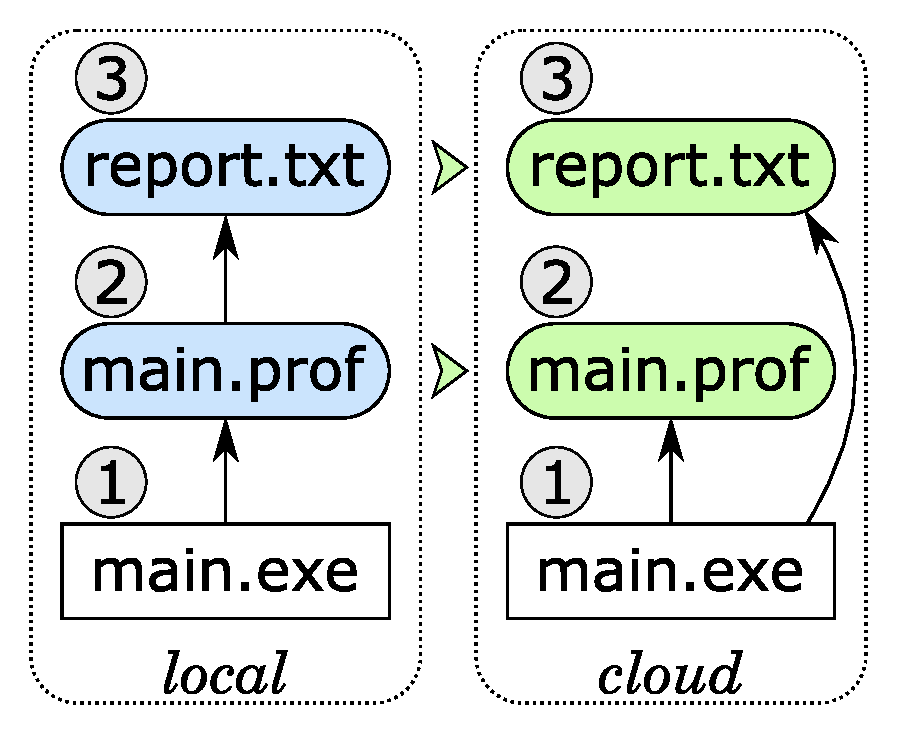
\includegraphics[scale=0.26]{fig/frankenbuild-example-build.pdf}}
% \vspace{-1.5mm}
\caption{Initial build}
\end{subfigure}
\begin{subfigure}[b]{0.32\linewidth}
\centerline{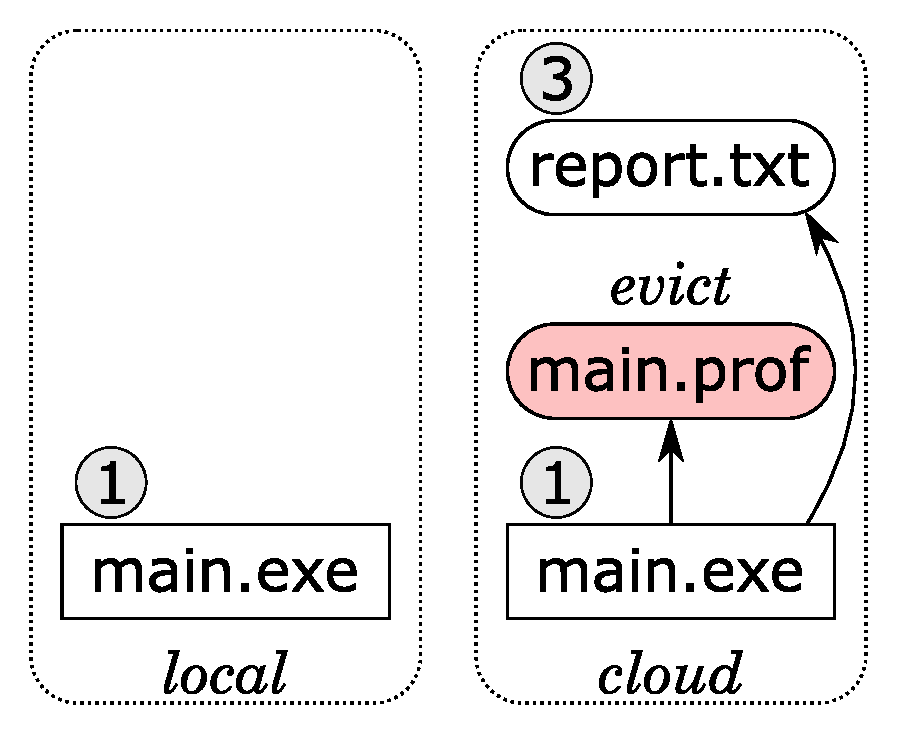
\includegraphics[scale=0.26]{fig/frankenbuild-example-clean.pdf}}
% \vspace{-1.5mm}
\caption{Clean up, evict \cmd{main.prof}}
\end{subfigure}
\begin{subfigure}[b]{0.34\linewidth}
\centerline{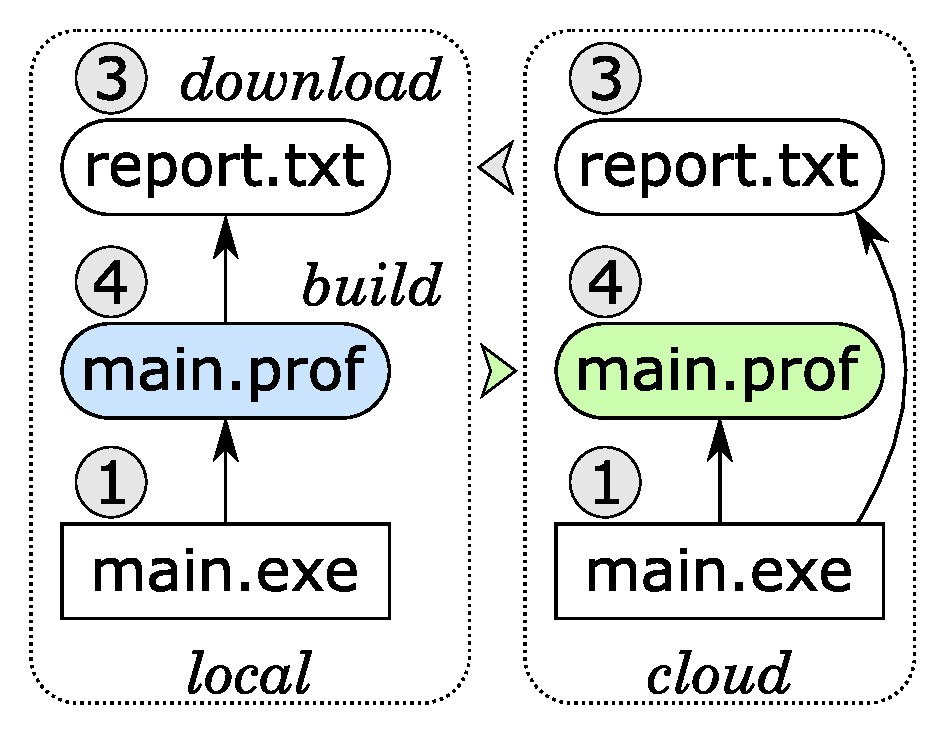
\includegraphics[scale=0.26]{fig/frankenbuild-example-rebuild.pdf}}
% \vspace{-1.5mm}
\caption{Build \cmd{main.prof} \& \cmd{report.txt}}
\end{subfigure}
% \vspace{-1.5mm}
\caption{A Frankenbuild example: (a)~build a human-readable profiling report for
\cmd{main.exe} from information dump \cmd{main.prof} produced by a profiling
tool, then record deep constructive traces in the cloud, (b)~remove built files
locally and evict \cmd{main.prof} from the cloud storage, (c)~build
\cmd{main.prof} by executing the profiler (profiling is non-deterministic, hence
the new hash value), then build \cmd{report.txt} by downloading it from the
matching deep constructive trace in the cloud, resulting in a Frankenbuild
because \cmd{main.prof} and \cmd{report.txt} are inconsistent. New and evicted
cloud storage entries are highlighted; file hashes are shown in circles.
\label{fig-frankenbuild}}
% \vspace{-4mm}
\end{figure}

Deep constructive traces (\S\ref{sec-deep-constructive-traces}) combined with
task non-determinism (\S\ref{sec-non-determinism}) can lead to very subtle bugs,
especially in the cloud setting. Fig.~\ref{fig-frankenbuild} shows a
\emph{Frankenbuild}~\cite{esfahani2016cloudbuild} example, where the target
\cmd{report.txt}, which is downloaded from the cloud, is inconsistent with its
immediate dependency \cmd{main.prof}. This inconsistency is caused by two factors:
(i)~inherent non-determinism of profiling: running a profiling tool on the very
same \cmd{main.exe} will produce different \cmd{main.prof} results every time;
and (ii)~relying on deep constructive traces, which cache build results based
only on the hashes of terminal task inputs (in this case \cmd{main.exe}). Note
that the resulting store is incorrect according to all three definitions of
correctness: the main definition~(\S\ref{sec-build-correctness}), the variant
for non-deterministic tasks~(\S\ref{sec-non-determinism}) and the variant for
shallow builds~(this section).

\todo{AM/NM}{Re-using existing infrastructure: (a) key-value store, (b) remote execution service.}

\subsection{Self-tracking}\label{sec-tracking-aspects}

Some build systems, for example \Excel and \Ninja, are capable of recomputing a
task if either its dependencies change, \emph{or} the task itself changes. For
example:

\vspace{0.5mm}
\begin{minted}[xleftmargin=10pt]{text}
A1 = 20      B1 = A1 + A2
A2 = 10
\end{minted}
\vspace{0.5mm}

\noindent
In \Excel the user can alter the value produced by \cmd{B1} by either editing
the inputs of \cmd{A1} or \cmd{A2}, \emph{or} editing the formula in
\cmd{B1}~--~e.g. to \cmd{A1 * A2}. This pattern can be captured by describing
the rule producing \cmd{B1} as also depending on the value \cmd{B1-formula}.
The implementation can be given very directly in a
\hs{Tasks}~\hs{Monad}~--~concretely, first look up the formula, then interpret
it:

\vspace{0.5mm}
\begin{minted}[xleftmargin=10pt]{haskell}
sprsh4 "B1" = Just $ Task $ \fetch -> do
    formula <- fetch "B1-formula"
    evalFormula fetch formula
\end{minted}
\vspace{0.5mm}

\noindent
The build systems that have precise self-tracking are all ones which use a
\emph{non-embedded domain specific language} to describe build tasks. Those
which use a full programming language, e.g. \Shake, are faced with the challenge
of implementing equality on arbitrary task functions. For such build systems,
the pessimistic assumption that any change to the build system potentially
changes any build task can often be used~--~the classic example being a makefile
depending on itself.

\todo{AM}{Self-tracking (?):
  https://github.com/snowleopard/build/blob/master/src/Build/SelfTracking.hs}


\subsection{Iterative Computations}\label{sec-iterative-compute}

Some computations are best described not by a chain of acyclic dependencies,
but by a loop. For example, \LaTeX~requires repeated rebuilding until it
reaches a fixed point, which can be directly expressed in build systems, such as
\Pluto~\cite{erdweg2015pluto}. Another example is \Excel, where a cell can
depend on itself, for example: \cmd{A1 = A1 + 1}. In such cases \Excel will
normally not execute anything, but if the ``Iterative Calculations'' feature is
enabled \Excel will execute the formula for a specified maximum number $N$ of
times per calculation (where $N$ is a setting that defaults to 100).

For examples like \LaTeX~we consider the proper encoding to not be circular
tasks, but a series of iterative steps, as described
by~\cite{shake-fixed-point}. It is important that the number of executions is
bounded, otherwise the build system may not terminate (a legitimate concern
with \LaTeX, which can be put into a situation where it is bistable or diverging
over multiple executions). The examples in \Excel tend to encode either mutable
state, or recurrence relations. The former is only required because \Excel
inherently lacks the ability to write mutable state, and the latter is probably
better solved using explicit recurrence formulae.

Overall we choose not to deal with cyclic dependencies, a choice that most build
systems also follow. There are computation frameworks that support tasks with
cyclic dependencies under the assumption that tasks are \emph{monotonic} in a
certain sense, e.g. see~\cite{pottier2009lazy} and~\cite{radul2009propagation}.

\subsection{Polymorphism}\label{sec-polymorphism}

Our build system abstraction assumes a \hs{k}/\hs{v} store, along with a build
system that works directly on \hs{k} and \hs{v} values. However, some build
systems provide greater flexibility, e.g. \Shake permits polymorphic keys and
values, allowing types that are stored only in the \Shake's build information.

As one example of richer key/value types, consider the version of
\cmd{gcc}~--~for many builds it should be a dependency. In \Shake it is possible
to define an \emph{oracle} rule as per~\cite{mitchell2012shake} whose value is
the result of running \cmd{gcc -}\cmd{-version} and which is volatile, making the
\cmd{gcc} version something that can be depended upon. Of course, provided the
build can express volatile dependencies and supports cutoff, the version number
could equally be written to a file and used in a similar way.

A more compelling example is build tasks that produce multiple output
keys~--~for example, \cmd{ghc Foo.hs} produces both \cmd{Foo.hi} and \cmd{Foo.o}.
That can be represented by having a key whose value is a pair of file names, and
whose result is a pair of file contents. From that, the task for \cmd{Foo.hi}
can be the first component of the result of the pair. Again, such an operation
can be encoded without polymorphic keys provided the pair of files (or a dummy
file representing the pair) is marked as changed if either of the contained
files change. Once again, polymorphic dependencies provide convenience rather
than power.

\Shake users have remarked that polymorphism provides a much easier expression
of concepts, e.g.~\cite{hadrian}, but it is not essential and we therefore do
not model it in this paper\footnote{See modules \cmd{Build.Multi} and
\cmd{Build.Task.Typed} in our framework for models of multiple-output and
polymorphic tasks.}.

\todo{AM}{Tasks with multiple outputs:
  https://github.com/snowleopard/build/blob/master/src/Build/Multi.hs}

\todo{AM}{Typed tasks:
  https://github.com/snowleopard/build/blob/master/src/Build/Task/Typed.hs}

\section{Related Work}\label{sec-related}

While there is research on individual build systems, there has been little
research to date comparing different build systems. In~\S\ref{sec-background} we
covered several important build systems~--~in this section we relate a few
other build systems to our abstractions, and discuss other work where similar
abstractions~arise.

\subsection{Other Build Systems}\label{sec-related-build}

Most build systems, when viewed at the level we talk, can be captured with minor
variations on the code presented in \S\ref{sec-implementations}. Below we list
some notable examples:

\begin{itemize}
\item \Dune~\cite{dune} is a build system designed for OCaml/Reason projects.
Its original implementation used \emph{arrows}~\cite{hughes2000generalising}
rather than monads to model dynamic dependencies, which simplified static
dependency approximation. \Dune was later redesigned to use a flavour of
selective functors~\cite{mokhov_selective_2019}, making it a closer fit to our
abstractions.

\item \Ninja~\cite{ninja} combines the \hs{topological} scheduler of \Make with
the verifying traces of \Shake~--~our associated implementation provides such a
combination. \Ninja~is also capable of modelling build rules that produce
multiple results, a limited form of multiple value types \S\ref{sec-polymorphism}.

\item \Nix~\cite{dolstra2004nix} has coarse-grained dependencies, with precise
hashing of dependencies and downloading of precomputed build products. We
provided a model of \Nix in \S\ref{sec-implementation-cloud}, although it is
worth noting that \Nix is not primarily intended as a build system, and the
coarse grained nature (packages, not individual files) makes it targeted to a
different purpose.

\item \Pluto~\cite{erdweg2015pluto} is based on a similar model to \Shake, but
additionally allows cyclic build rules combined with a user-specific resolution
strategy. Often such a strategy can be unfolded into the user rules without loss
of precision, but a fully general resolution handler extends the \hs{Task}
abstraction with new features.

\item \Redo~\cite{redo-idea,grosskurth2007redo,redo} almost exactly
matches \Shake at the level of detail given here, differing only in aspects like
rules producing multiple files~\S\ref{sec-polymorphism}. While \Redo predates
\Shake, they were developed independently; we use \Shake as a prototypical
example of a monadic build system because its implementation presents a closer
mapping to our \hs{Task} abstraction.

\item \Tup~\cite{tup} functions much like \Make, but with a refined dirty-bit
implementation that watches the file system for changes and can thus avoid
rechecking the entire graph. \Tup also automatically deletes stale results.
\end{itemize}

The one build system we are aware of that cannot be modelled in our framework is
\Fabricate by~Hoyt~\etal~\shortcite{fabricate}. In \Fabricate a build system is
a script that is run in-order, in the spirit of:

\vspace{1mm}
\begin{minted}[xleftmargin=10pt]{bash}
gcc -c util.c
gcc -c main.c
gcc util.o main.o -o main.exe
\end{minted}
\vspace{1mm}

% \noindent
To achieve minimality, each separate command is traced at the OS-level, allowing
\Fabricate to record a trace entry stating that \cmd{gcc -c util.c} reads from
\cmd{util.c}. In future runs \Fabricate runs the script from start to finish,
skipping any commands where no inputs have changed. The main difference from our
\hs{Tasks} abstraction is that instead of supplying a mapping from keys to
tasks, a \Fabricate script supplies a list of build statements, in a
\emph{user-scheduled order}, without declaring what each statement reads or write.

Taking our abstraction, it is possible to encode \Fabricate assuming that
commands like \cmd{gcc -c util.c} are keys, there is a linear dependency between
each successive key, and that the OS-level tracing can be lifted back as a
monadic \hs{Task} function\footnote{\Shake provides support for
\Fabricate{}-like build systems~--~see \cmd{Development.Shake.Forward}.}.
However, in our pure model the mapping is not perfect as \cmd{gcc} writes to
arbitrary files whose locations are not known in advance. One way of capturing
arbitrary writes in our model is to switch from one callback \hs{fetch} to
\emph{two callbacks}, say \hs{read} and \hs{write}, allowing us to track both
reads and writes separately.

\subsection{Self-adjusting Computation}

While not typically considered build systems, self-adjusting computation is a
well studied area, and in particular the contrast between different formulations
has been thoroughly investigated, e.g.
see~Acar~\etal~\shortcite{acar2007selfadjusting}. Self-adjusting computations
can automatically adjust to an external change to their inputs. A classic
example is a self-adjusting sorting algorithm, which can efficiently (in
$O(\log{n})$ time where $n$ is the length of the input) recalculate the result
given an incremental change of the input. While very close to build systems in
spirit, self-adjusting computations are mostly used for in-memory computation
and rely on the ability to dynamically allocate new keys in the store for
sharing intermediate computations~--~an intriguing feature rarely seen in build
systems (\Shake's oracles~\S\ref{sec-polymorphism} can be used to model this
feature to a limited degree). Another important optimisation that self-adjusting
computation engines often support is the incremental processing of
\emph{deltas}, where instead of marking a value as ``changed to 8'', one can
mark it as ``changed by $+1$'', assuming it was equal to 7 before. When a delta
is small, it can often be propagated to the output more efficiently than by
recomputing the output value from scratch.

A lot of research has been dedicated to finding efficient data structures and
algorithms for self-adjusting computations, with a few open-source
implementations, e.g. \Incremental by Jane Street~\shortcite{incremental}. We
plan to investigate how these insights can be utilised by build systems as
future work.

\subsection{Memoization}\label{sec-related-memo}

\emph{Memoization} is a classic optimisation technique for storing values of a
function instead of recomputing them each time the function is called. Minimal
build systems (\S\ref{sec-background-make}) certainly perform
memoization: they \emph{store values instead of recomputing them each time}.
Memoization can therefore be reduced to a minimal build system (as we
demonstrate below), but not vice versa, since minimal build systems solve a more
complex optimisation problem.

As a simple example of using a build system for memoization, we solve a textbook
dynamic programming problem~--~Levenshtein's \emph{edit
distance}~\cite{levenshtein1966binary}: given two input strings $a$ and
$b$, find the shortest series of edit operations that transforms $a$
to $b$. The edit operations are typically \emph{inserting}, \emph{deleting} or
\emph{replacing} a symbol. The dynamic programming solution of this problem is
so widely known, e.g., see~Cormen~\etal~\shortcite{cormen2001introduction}, that
we provide its encoding in our \hs{Tasks} abstraction without further
explanation. We address elements of strings $a_i$ and $b_i$ by keys \hs{A}~$i$
and \hs{B}~$i$, respectively, while the cost of a subproblem $c_{ij}$ is
identified by \hs{C}~$i$~$j$.

\vspace{1mm}
\begin{minted}[xleftmargin=10pt]{haskell}
data Key = A Int | B Int | C Int Int deriving Eq
\end{minted}
\begin{minted}[xleftmargin=10pt]{haskell}
editDistance :: Tasks Monad Key Int
editDistance (C i 0) = Just $ Task $ const $ pure i
editDistance (C 0 j) = Just $ Task $ const $ pure j
editDistance (C i j) = Just $ Task $ \fetch -> do
    ai <- fetch (A i)
    bj <- fetch (B j)
    if ai == bj
        then fetch (C (i - 1) (j - 1))
        else do
            insert  <- fetch (C  i      (j - 1))
            delete  <- fetch (C (i - 1)  j     )
            replace <- fetch (C (i - 1) (j - 1))
            return (1 + minimum [insert, delete, replace])
editDistance _ = Nothing
\end{minted}
\vspace{1mm}

\noindent
When asked to build \hs{C}~$n$~$m$, a minimal build system will calculate the
result using memoization. Furthermore, when an input $a_i$ is changed, only
necessary, incremental recomputation will be performed~--~an optimisation that
cannot be achieved just with memoization.

Self-adjusting computation, memoization and build systems are inherently related
topics, which poses the question of whether there is an underlying common
abstraction waiting to be discovered.

\section{Conclusions}\label{sec-conclusions}

We have investigated multiple build systems, showing how their properties are consequences of two implementation choices: what order you build in and how you decide whether to rebuild. By first decomposing the pieces, we show how to recompose the pieces to find new points in the design space. In particular, a simple recombination leads to a design for a monadic suspending cloud build system, which we have implemented and use in our day-to-day development.


\bibliography{refs}

\appendix
% \clearpage
\section{Appendix}\label{sec-appendix}

\subsection{Compute transformers}\label{sec-appendix-transformers}

In this section we clarify some of the compute transformers used in this paper.

\hs{execute} uses the transformation based on the \hs{Identity} monad, feeding
\hs{fetch k = pure (store k)} to the compute:

\begin{minted}[xleftmargin=10pt]{haskell}
execute :: Compute Monad k v -> (k -> v) -> k -> Maybe v
execute compute store = fmap runIdentity . compute (pure . store)
\end{minted}
\vspace{1mm}
\begin{minted}[xleftmargin=10pt]{haskell}
newtype Identity a = Identity { runIdentity :: a }
\end{minted}
\vspace{1mm}
\begin{minted}[xleftmargin=10pt]{haskell}
instance Functor Identity where
    fmap f (Identity a) = Identity (f a)
\end{minted}
\vspace{1mm}
\begin{minted}[xleftmargin=10pt]{haskell}
instance Applicative Identity where
    pure a = Identity a
    Identity f <*> Identity a = Identity (f a)
\end{minted}
\vspace{1mm}
\begin{minted}[xleftmargin=10pt]{haskell}
instance Monad Identity where
    Identity a >>= f = f a
\end{minted}
\vspace{1mm}

\todo{AM}{Explain \hs{track}.}



Here is a draft implementation of \hs{inputs} used in the definition of
build system correctness in \S\ref{sec-build-correctness}:

\begin{minted}[xleftmargin=10pt]{haskell}
inputs :: Eq k => Task Monad k v -> Store i k v -> k -> [k]
inputs task store key = filter (isInput task) (closure deps key)
  where
    deps k = maybe [] snd (track task (\k -> getValue k store) k)

closure :: Eq a => (a -> [a]) -> a -> [a] -- Standard graph transitive closure

data Proxy a = Proxy

isInput :: Task Monad k v -> k -> Bool
isInput task = isNothing . task (const Proxy)
\end{minted}

\subsection{Compute examples}\label{sec-appendix-compute-examples}

\todo{AM}{Add some explanatory text.}

The \emph{Collatz sequence} $C_i$ is defined as follows:

\[
C_{i} = {\begin{cases}~n&{\text{for }}i=0\\~f(C_{i-1})&{\text{otherwise}},\end{cases}}\hspace{12pt}\text{where}\hspace{12pt}f(k)={\begin{cases}~k/2&{\text{if }}k\text{ is even}\\~3k+1&{\text{otherwise}}\end{cases}}
\vspace{2mm}
\]
\noindent
and $n$ is a positive integer parameter. The famous \emph{Collatz conjecture}
states that the Collatz sequence eventually reaches 1 for all possible values of
$n$. For example, if $n=6$, we reach 1 in eight steps:
$(6, 3, 10, 5, 16, 8, 4, 2, 1, \dots)$, after which the sequence loops forever:
$(4, 2, 1, 4, 2, 1, \dots)$.

We can express the computation of values in the Collatz sequence as a functorial
compute:

\begin{minted}[xleftmargin=10pt]{haskell}
data Collatz = Collatz Int

collatz :: Compute Functor Collatz Int
collatz get (Collatz k) | k <= 0    = Nothing
                        | otherwise = Just $ f <$> get (Collatz (k - 1))
  where
    f n | even n    = n `div` 2
        | otherwise = 3 * n + 1
\end{minted}

...

The \emph{generalised Fibonacci sequence} $F_i$ is defined as follows:

\[
F_{i} = {\begin{cases}~n&{\text{for }}i=0\\~m&{\text{for }}i=1\\~F_{i-1}+F_{i-2}&{\text{otherwise}}\end{cases}}
\vspace{2mm}
\]
\noindent
where $n$ and $m$ are integer parameters. By setting $n=0$ and $m=1$ we obtain
the famous \emph{Fibonacci sequence}: $(0, 1, 1, 2, 3, 5, 8, 13, \dots$), and if
$n=2$ and $m=1$, the result is the \emph{Lucas sequence}:
$(2, 1, 3, 4, 7, 11, 18, 29, \dots)$.

We can express the computation of values in the generalised Fibonacci sequence
as an applicative compute:

\begin{minted}[xleftmargin=10pt]{haskell}
data Fibonacci = Fibonacci Int

fibonacci :: Compute Applicative Fibonacci Int
fibonacci get (Fibonacci k) | k <= 1    = Nothing
                            | otherwise = Just $ (+) <$> get (Fibonacci (k - 1))
                                                     <*> get (Fibonacci (k - 2))
\end{minted}

...

The \emph{Ackermann function} $A(m, n)$ is defined as follows:

\[
A(m, n) = {\begin{cases}~n+1&{\text{for }}m=0\\~A(m-1, 1)&{\text{for }}n=0\\~A(m-1,A(m,n-1))&{\text{otherwise}}\end{cases}}
\vspace{2mm}
\]
\noindent
We can express the computation of the Ackermann function as a monadic compute:

\begin{minted}[xleftmargin=10pt]{haskell}
data Ackermann = Ackermann Int Int

ackermann :: Compute Monad Ackermann Int
ackermann get (Ackermann m n)
    | m < 0 || n < 0 = Nothing
    | m == 0    = Just $ return (n + 1)
    | n == 0    = Just $ get (Ackermann (m - 1) 1)
    | otherwise = Just $ do
        index <- get (Ackermann m (n - 1))
        get (Ackermann (m - 1) index)
\end{minted}

\end{document}
